\documentclass[10pt]{article}
\usepackage[a4paper, margin=2cm]{geometry} % 设置页面大小为A4,边距为2cm
\usepackage{hyperref}
\usepackage{graphicx}
\usepackage[style=numeric]{biblatex} % 例如使用数值样式
\addbibresource{references.bib} % 假设你的BibTeX文件名为references.bib
\usepackage{amsmath} % 数学公式宏包
\usepackage{listings} % 引入代码列表宏包
\usepackage{xcolor} % 引入颜色宏包
\usepackage{caption} % For captions in minipages
\usepackage{float}
\usepackage{fancyvrb}
\usepackage{color}
\usepackage[titletoc]{appendix}
\usepackage{adjustbox}
\usepackage{titling}



% 设置代码的样式
\lstset{
    language=Python, % 设置语言
    basicstyle=\ttfamily\small, % 基础代码风格
    keywordstyle=\color{blue}, % 关键词风格
    stringstyle=\color{red}, % 字符串风格
    commentstyle=\color{green}, % 注释风格
    morecomment=[l][\color{magenta}]{\#},
    frame=single, % 单框
    breaklines=true, % 自动换行
    numbers=left, % 行号在左侧
    numberstyle=\tiny\color{gray}, % 行号风格
    showstringspaces=false % 不显示字符串中的空格
}

% Define colors
\definecolor{darkred}{RGB}{139,0,0}
\definecolor{darkblue}{RGB}{0,0,139}

% Title page configuration
\title{
\includegraphics[width=0.3\textwidth]{../BirmCrest.png}\\
        \Huge{\textbf{Enhancing Online News Consumption with AI: The Development of Mirror News Summarizer}}
}
\author{{Zijun Li}\\[10pt]
        {\textbf{Student ID}: 2272583}\\[10pt]
        {BSc Computer Science}\\[10pt]
        {\textbf{Module Credits}: 40}\\[20pt]
        {\textbf{Supervisor}: Jizheng Wan}\\[10pt]
        {\textbf{Programme Name}: Mirror News Summarizer}\\[10pt]
        {\textbf{Word Count}: 6583}\\[20pt]
        {\textbf{Deployed Website}: \href{http://35.178.153.233:5000/}{http://35.178.153.233:5000/}}\\[10pt]
        {\textbf{GitLab Repository}: \href{https://git.cs.bham.ac.uk/projects-2023-24/zxl183}{https://git.cs.bham.ac.uk/projects-2023-24/zxl183}}\\[10pt]
}


\begin{document}
\begin{titlingpage} % Create a custom title page
    \setlength{\droptitle}{1em}    % Move title up
    \maketitle
    \thispagestyle{empty}
\end{titlingpage}

\newpage

\begin{center}
	\tableofcontents
	\addcontentsline{toc}{section}{Table of Contents}
\end{center}

\newpage

\begin{abstract}
    The "Mirror News Summarizer" project aimed to revolutionize the online news consumption experience by developing an advanced platform that streamlines information acquisition. Utilizing cutting-edge AI technologies, including NLP models for summarization and AI-driven recommendation systems, the platform offers succinct summaries of articles from selected news sites, maintaining a format reminiscent of the original. This design significantly reduces decision fatigue and enhances user engagement through personalized recommendations. The project's development process, grounded in cookiecutterflask, resulted in a Minimum Viable Product (MVP) that embodies efficient news reading with user-centric features like ad-free viewing. This report details the project's objectives, methodologies, implementation, and the iterative enhancements based on user feedback, showcasing its contribution to personalized and efficient news consumption in the digital age.
\end{abstract}

\section*{Acknowledgments}
\thispagestyle{empty} % No page number for the acknowledgment page

I would like to extend my sincerest gratitude to several key contributors and resources that have significantly aided the development of the "Mirror News Summarizer" project.

First and foremost, my appreciation goes to the BBC and Sky News for their exemplary standards in news reporting and their comprehensive and accessible online platforms. The structured and reliable content provided by these news outlets has been indispensable in the realization of this project, offering a rich source of data for summarization and analysis.

I am also profoundly thankful to the creators and maintainers of the Cookiecutter Flask project. The Cookiecutter Flask template has provided a robust and flexible foundation for building this application. Its well-structured and comprehensive framework significantly expedited the development process, allowing me to focus on the unique aspects of the news summarization features.

Furthermore, I extend my thanks to the open-source community for their invaluable resources, documentation, and forums. Their collective knowledge and willingness to share expertise have been a constant source of guidance and inspiration throughout this project's development.

Finally, I wish to acknowledge my supervisor, Jizheng Wan and inspector, Shan He for their guidance, support, and valuable insights that have greatly contributed to the success of this project.

\section{Motivation \& Aims}
The motivation behind the "Mirror News Summarizer" project is to address the challenge of information overload in digital news consumption. The project aims to create a platform that simplifies access to news by providing concise summaries, personalized content recommendations, and a user-friendly interface, thereby enhancing the efficiency and enjoyment of news reading in the digital era.

\subsection{General problem}
Expanding on the general problem of information overload in the digital age, recent statistics and studies provide a clearer understanding of this phenomenon. A Pew Research Center survey indicates that a majority of Americans engage with news across multiple platforms, with 67\% using news websites or apps, and a significant portion, 49\%, utilizing social media for news consumption \cite{pewnewsplatforms} . This digital news consumption is predominant among younger demographics, particularly those aged 18-29, who prefer digital devices over traditional media \cite{pewnewsplatforms} .

The issue is not just the volume of information but its impact on consumers. Research suggests that news overload on social media leads to exhaustion and indifference towards news \cite{frontiersinpsych2022} . The fast pace of information dissemination through mobile devices and constant updates exacerbates this problem, increasing the demand on cognitive resources and leading to a phenomenon known as "news avoidance," where consumers deliberately avoid news to reduce stress and cognitive load \cite{frontiersinpsych2022} .

This backdrop of overwhelming digital news consumption and its effects forms the basis for addressing the specific problem tackled by the "Mirror News Summarizer" project. 

\subsection{Significance of the Problem}
Building on the impact of information overload on users, it's worth highlighting the broader implications of this issue on society's collective ability to stay informed. The relentless influx of information can not only overwhelm individual users but also affect public discourse and the quality of democratic engagement. When users are bombarded with too much information, they may retreat into echo chambers or engage in selective exposure to information, reinforcing existing biases and reducing exposure to diverse viewpoints.

The phenomenon of decision fatigue further exacerbates this issue. Faced with an overwhelming array of choices and information, individuals may become less capable of making informed decisions or even opting to disengage from news consumption altogether. This trend poses significant challenges for the fabric of informed citizenship.

Although specific statistics detailing the full extent of these societal impacts are complex to pin down, research from the Pew Research Center and other organizations indicates that a substantial portion of the population feels overwhelmed by the amount of information available. For instance, Pew's findings that 20\% of Americans report feeling overloaded by information highlight the personal impact, but the societal implications—such as decreased civic engagement or increased polarization due to selective exposure—though harder to quantify, are of great concern \cite{pewnewsplatforms} .

Additionally, the role of social media in news consumption adds another layer of complexity. Platforms designed to capture and retain user attention often prioritize engaging content over informative content, potentially skewing public perception and understanding of important issues  \cite{frontiersinpsych2022} . The rapid dissemination of misinformation through these channels further complicates the landscape, making the need for effective tools to manage information overload and enhance the quality of news consumption even more pressing.

In sum, the significance of addressing information overload extends beyond individual user experience to encompass broader societal impacts. By developing solutions like the "Mirror News Summarizer," there's potential not only to improve individual well-being by reducing information overload and decision fatigue but also to contribute positively to the quality of public discourse and democratic processes.

\subsection{Prior Work on the Problem}
In addressing the problem of information overload in news consumption, several platforms have emerged with innovative solutions. Inshorts\cite{inshorts2018}, for example, distills news into concise 60-word summaries, appealing to users seeking quick updates. Feedly\cite{feedlyFeatures} offers a more customizable experience, allowing users to aggregate news from preferred sources into a single feed, enhancing control over the information influx. Flipboard\cite{flipboardMagazine} combines these approaches with a visually engaging format, presenting news in a magazine-like layout that prioritizes user interests and visual storytelling.

Despite these advancements, gaps remain in the existing solutions. While these platforms have pioneered the use of algorithms for summarization and personalization, they often rely heavily on user input for customization, which can itself become a source of overload. Moreover, the challenge of maintaining a distraction-free reading environment amidst the monetization strategies that include advertisements and sponsored content has not been fully addressed. The emphasis on visual engagement by platforms like Flipboard\cite{flipboardMagazine}, although aesthetically pleasing, sometimes detracts from the core goal of simplifying news consumption and can still contribute to cognitive overload.

To enhance the persuasiveness of this discussion, it's pertinent to consider additional examples and scholarly insights. Studies indicate that while digital platforms have made news more accessible, the sheer volume and rapid pace of updates can deter users from engaging deeply with content, leading to superficial understanding or avoidance behaviors  \cite{frontiersinpsych2022} . This underscores the need for solutions that not only condense and curate content but also present it in a way that encourages deeper engagement without overwhelming the user.

\subsection{Specific Problem}
The "Mirror News Summarizer" project endeavors to confront the nuanced challenges of modern news consumption by integrating AI-driven summarization with an intuitive, user-focused design. Its ambition is to bridge the divide between the volume of available news and the cognitive capacity of users to process this information. By synthesizing news articles into concise summaries and reflecting the original site's layout, the project aims to reduce cognitive load, preserving the user's comfort with familiar formats while streamlining their reading experience.

This endeavor acknowledges the critical feedback from existing platforms, where personalization often requires extensive user input, leading to potential information overload. The "Mirror News Summarizer" intends to leverage advanced machine learning algorithms to analyze user behavior and preferences subtly, thereby offering a more adaptive and personalized news feed without necessitating active user customization. This intelligent personalization seeks to present users with content that is not only relevant but also curated in a way that respects their time and attention span.

Furthermore, the project is committed to creating a distraction-free environment, recognizing that advertisements and pop-ups significantly detract from the quality of the user experience. By eliminating these interruptions, the "Mirror News Summarizer" aspires to foster a more focused and enjoyable reading journey, allowing users to engage with news content without the typical barriers that might discourage deep reading.

\newpage
\section{Methodology}

\subsection{Intention}
The "Mirror News Summarizer" project is dedicated to crafting a platform that addresses the prevalent challenge of information overload in today's digital news landscape. Central to our mission is the design of a news reading experience that is not only efficient and personalized but also deeply familiar to users. By leveraging artificial intelligence (AI) to distill lengthy news articles into precise summaries, we have been meticulous in mirroring the aesthetic and structural layout of original news websites. This meticulous emulation of design elements serves as a cornerstone of the platform, as it reduces cognitive load and fosters a seamless transition between traditional news reading and our streamlined summaries.

This focus on creating a user-centric platform stems from a recognition of the cognitive demands associated with sifting through abundant news content. By maintaining the look and feel of traditional news sites, the "Mirror News Summarizer" offers users a comforting sense of familiarity, which is crucial for enhancing readability and retaining the essence of the news experience. Such design philosophy ensures that users can consume news quickly and effortlessly while still enjoying an environment that mirrors their preferred news outlets.

\subsection{Approach}
The methodology of the "Mirror News Summarizer" project is rooted in a multi-faceted approach combining data acquisition, artificial intelligence (AI), and user experience design to address the specific challenges identified.

\subsubsection{Data Acquisition and Processing}
The first step involves collecting news articles from various reputable sources. This process is facilitated through web scraping techniques that provide access to a wide range of news content. The selection of sources is guided by credibility and diversity to ensure a comprehensive news feed. The acquired data undergo preprocessing to normalize text format and remove any non-essential elements like advertisements or multimedia elements that do not contribute to the core news narrative.

For web scraping, Python's BeautifulSoup and Requests libraries are employed to navigate and extract relevant news content. JSON parsing is used to retrieve and organize data. 


\textbf{Extracting Navigation Data from HTML Content:}
This process begins by taking the input HTML content and converting it into a BeautifulSoup object for parsing. The primary task is to extract the main and secondary navigation data from the HTML.\ref{fig:navbar}
    
\begin{enumerate}
    \item Firstly, the script checks for the presence of the main navigation container within the HTML structure. If found, it iterates over each list item (`li' tag) within the container. For each item, it attempts to find an anchor (`a' tag) with a specific class indicating a link. If the anchor tag is present and contains an `href' attribute, the script constructs a relative navigation URL.
    \item Subsequently, it searches for a span containing the title within each anchor tag. The extracted URL and title are then appended to a list, which represents the entire navigation structure.
    \item Finally, the script returns this list of navigation links and compiles all extracted information into a single output.
\end{enumerate}
\textbf{Example Output:}
\begin{lstlisting}
return {
    'news': "BBC",
    'nav': nav,
    'nav_secondary': nav_secondary,
    'timestamp': current_time.strftime('%Y-%m-%d %H:%M:%S'),
}        
\end{lstlisting}

\textbf{Homepage Data Extraction Process:}
The function \textit{extract\_data\_sky\_news\_homepage} orchestrates the extraction of structured news data from the given HTML content of Sky News. The process involves several steps to ensure the retrieval of relevant information, including article images, URLs, titles, authors, and news clusters.\ref{fig:maincontent}

\begin{enumerate}
    \item The HTML content is parsed into a BeautifulSoup object for convenient data navigation.
    \item Individual extraction functions like \textit{extract\_img\_url}, \textit{extract\_news\_url\_and\_title}, and \textit{extract\_most\_read\_news\_url\_and\_title} are employed to pull specific elements from the HTML structure.
    \item The \textit{extract\_clusters} function assembles news articles into clusters, distinguishing between most read articles and others based on the section headers.
    \item Lastly, a comprehensive data structure is returned, encapsulating the 'news' source, an array of 'clusters' containing articles, a 'timestamp' of the extraction time, and the 'url' of the homepage.
\end{enumerate}
\textbf{Example Output:}
\begin{lstlisting}
return {
    'news': "Sky",
    'clusters': clusters,
    'timestamp': current_time.strftime('%Y-%m-%d %H:%M:%S'),
    'url': url,
}
\end{lstlisting}

\begin{figure}[htbp]
    \centering
    \begin{minipage}[t]{0.35\textwidth}
        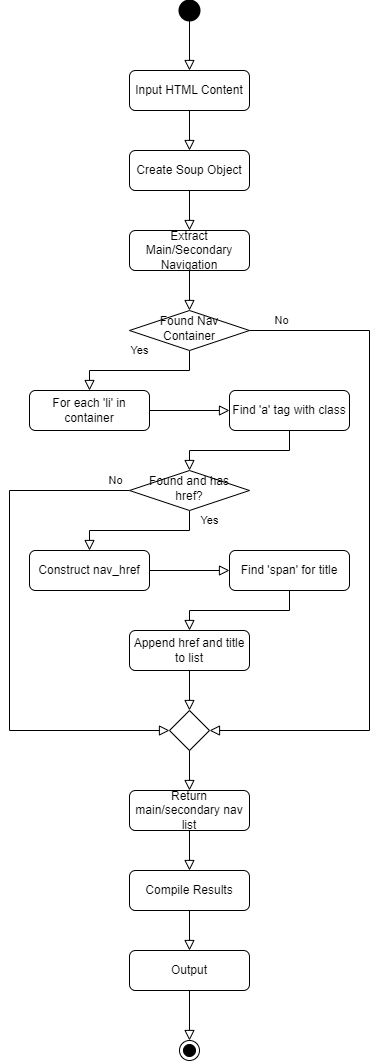
\includegraphics[width=\textwidth]{../FlowChart_Navbar.png}
        \caption{Navigation Data Extraction Process}
        \label{fig:navbar}
    \end{minipage}
    \hfill
    \begin{minipage}[t]{0.4\textwidth}
        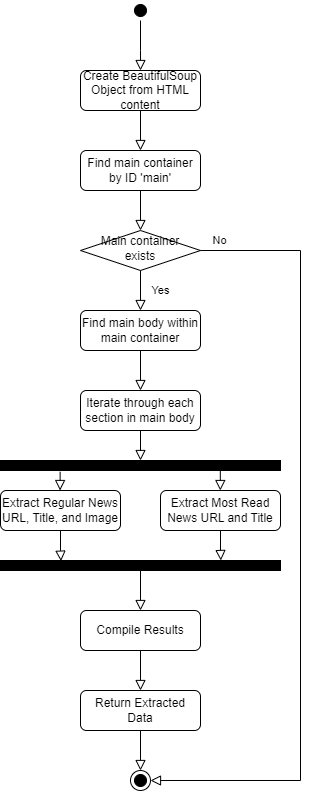
\includegraphics[width=\textwidth]{../FlowChart_Main.png}
        \caption{Mainpage Content Extraction Process}
        \label{fig:maincontent}
    \end{minipage}
    \hfill
\end{figure}

\begin{figure}[htbp]
    \centering
    \begin{minipage}[t]{0.35\textwidth}
        \raisebox{-\height}{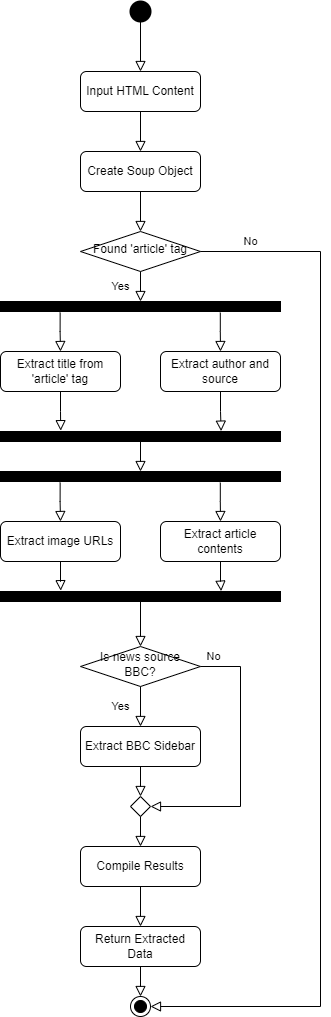
\includegraphics[width=\textwidth]{../FlowChart_Content.png}}
        \caption{Ariticle Content Extraction Process}
        \label{fig:newscontent}
    \end{minipage}
    \hfill
    \begin{minipage}[t]{0.6\textwidth}
    \textbf{Data Extraction Process for News Content:}
    The \textit{extract\_data\_news\_content} function is designed to parse the HTML content of a BBC News article and extract valuable information including the article title, author, and main content sections.\ref{fig:newscontent}

    \begin{enumerate}
        \item Parse the HTML content into a navigable object for easy querying (`soup`).
        \item Look for specific HTML tags (`article`, `div`, etc.) and extract relevant content (titles, authors, URLs, etc.).
        \item Assemble the extracted data into structured Python dictionaries, lists, or other suitable data types.
        \item Combine all pieces of extracted information into a single dictionary representing the article.
        \item Return the dictionary with all the extracted and compiled article data.
    \end{enumerate}

    \textbf{Sample Output Structure:}
    \begin{lstlisting}
return {
    'news': "BBC",
    'title': title,
    'content': ' '.join(section['content'] for section in sections), 
    'img_urls': img_urls if img_urls else '', 
    'url': url,
    'timestamp': current_time,
    'article_infos': {
        'author': author,
        'source': source,
        'date': None
    },
    'bbc_parts': {
        'related_topics': related_topics,
        'more_on_this_story': more_on_this_storys,
    },
    'sky_parts': {}, 
}
    \end{lstlisting}
    \end{minipage}
\end{figure}

\newpage

\subsubsection{AI-driven Summarization}
Upon preprocessing, the project focuses on employing AI models for the generation of concise summaries of news articles. Specifically, we leverage the capabilities of the ChatGPT API, a cutting-edge model based on the Transformer architecture, renowned for its performance in Natural Language Processing (NLP) tasks. Unlike traditional summarization models, ChatGPT's advanced understanding and generation capabilities allow it to identify and condense the key points of news articles into succinct summaries without losing the essence of the content. 

The decision to utilize ChatGPT over other available APIs is based on several key factors that align with our project's goals of efficiency and effectiveness in summarization tasks. The following table compares ChatGPT with other notable APIs based on criteria such as performance, ease of integration, and linguistic capabilities:

\begin{table}[H]
    \centering
    \begin{tabular}{lccc}
    \hline
    \textbf{Criteria} & \textbf{ChatGPT} & \textbf{BART} & \textbf{T5} \\ \hline
    Performance & High & High & High \\
    Ease of Integration & High & Medium & Medium \\
    Linguistic Capabilities & Advanced & Advanced & Advanced \\
    Real-time Processing & Yes & Yes & Yes \\
    Cost-Effectiveness & High & Medium & Medium \\ \hline
    \end{tabular}
    \caption{Comparison of Summarization APIs}
\end{table}
    
As illustrated, ChatGPT stands out due to its superior performance, especially in handling complex linguistic structures and generating coherent, contextually relevant summaries. Additionally, its ease of integration and cost-effectiveness make it an ideal choice for our project. In contrast, other APIs might offer real-time processing but fall short in terms of linguistic capabilities and overall summarization quality. Therefore, by leveraging ChatGPT, we aim to provide users with high-quality, efficient news summaries that cater to their interests and reading preferences.

\begin{lstlisting}
def get_summary(text, model="gpt-3.5-turbo", max_tokens=200):
    """
    This function takes a piece of text and returns its summary using OpenAI's chat model API.
    
    :param text: The text to summarize.
    :param model: The chat model to use for summarization.
    :param max_tokens: The maximum number of tokens to generate for the summary.
    :return: The summary of the text.
    """
    try:
        response = openai.ChatCompletion.create(
            model=model,
            messages=[{"role": "system", "content": "Summarize the following article:"},
                      {"role": "user", "content": text}],
            max_tokens=max_tokens
        )
        summary = response['choices'][0]['message']['content']
        return summary
    except openai.error.OpenAIError as e:
        # Handle the OpenAI API error appropriately
        print(f"An error occurred: {e}")
        return "An error occurred while generating the summary."
\end{lstlisting}

\newpage
\textbf{Text Summarization Process:}
The process involves taking a piece of text and generating a concise summary using OpenAI's GPT model via the API. 

\begin{enumerate}
    \item \textbf{Prepare the Input Text:} The text that needs to be summarized is prepared and passed to the \textit{get\_summary} function along with the model choice and the maximum token limit for the summary.
    
    \item \textbf{API Request Construction:} An API request is constructed with the text, specifying the role of the text as ``user" content and setting a system message to instruct the model to ``Summarize the following article:".
    
    \item \textbf{Invoke OpenAI's ChatCompletion API:} The constructed request is sent to OpenAI's ChatCompletion API, specifying the chosen model (e.g., ``gpt-3.5-turbo") and the maximum number of tokens for the summary.
    
    \item \textbf{Process API Response:} The API responds with a summary generated by the model. The response is processed to extract the summary text from the structured response data.
    
    \item \textbf{Error Handling:} If an error occurs during the API call (e.g., network issues, API limits), the error is caught, and an appropriate error message is returned instead of a summary.
    
    \item \textbf{Return the Summary:} The generated summary is returned to the calling function, ready to be used as a concise representation of the original text.
\end{enumerate}

This streamlined process efficiently condenses lengthy text into succinct summaries, leveraging the advanced capabilities of OpenAI's GPT models.

\subsubsection{Database Storage and Retrieval}

The "Mirror News Summarizer" project is underpinned by a robust database design, central to which is the \textbf{Articles} entity. This entity is the repository for all news content, acting as the mainstay for both the summarization process and user delivery. It is expansively constructed to integrate seamlessly with the various structural components unique to different news providers.\ref{fig:article db structure}

\paragraph{Core Attributes}
The foundational \textit{Articles} table within the database comprises the following attributes essential to each news article:
\begin{itemize}
    \item \textit{id} -- a unique identifier to manage and reference each article.
    \item \textit{title} -- the headline encapsulating the core message.
    \item \textit{content} -- the full narrative body of the news.
    \item \textit{summary} -- the algorithm-generated abridged version of the content.
    \item \textit{url} -- the URL to the original news article, ensuring credibility and reference continuity.
    \item \textit{timestamp} -- the time when the article was added to the system, crucial for timeline management.
\end{itemize}

\paragraph{Integration with Parts}
To accommodate the diversity of news formats, the database includes \textit{Parts} that reflect specific attributes of various news outlets. These are interconnected with the \textit{Articles} via a one-to-many relationship to enhance the contextual framework of the news content:
\begin{itemize}
    \item \textit{BBCPart} -- comprises identifiers that link the articles to BBC's unique features like sidebar content and related topics.
    \item \textit{SkyPart} -- connects the articles to thematic clusters as categorized by Sky News, mirroring its content organization.
\end{itemize}

The \textit{Parts} extend beyond mere association; they are essential in the recreation of a news-reading experience that is both authentic and user-friendly. The user reads the summary within an interface that reflects the familiar layout and style of the original news source.

The successful execution of this structure relies on adept database operations, specifically tailored \textit{join} operations that merge the \textit{Articles} with their respective \textit{Parts}. The database schema is optimally designed to handle these operations, ensuring prompt and accurate news delivery to the user interface.

\begin{figure}[H]
    \centering
    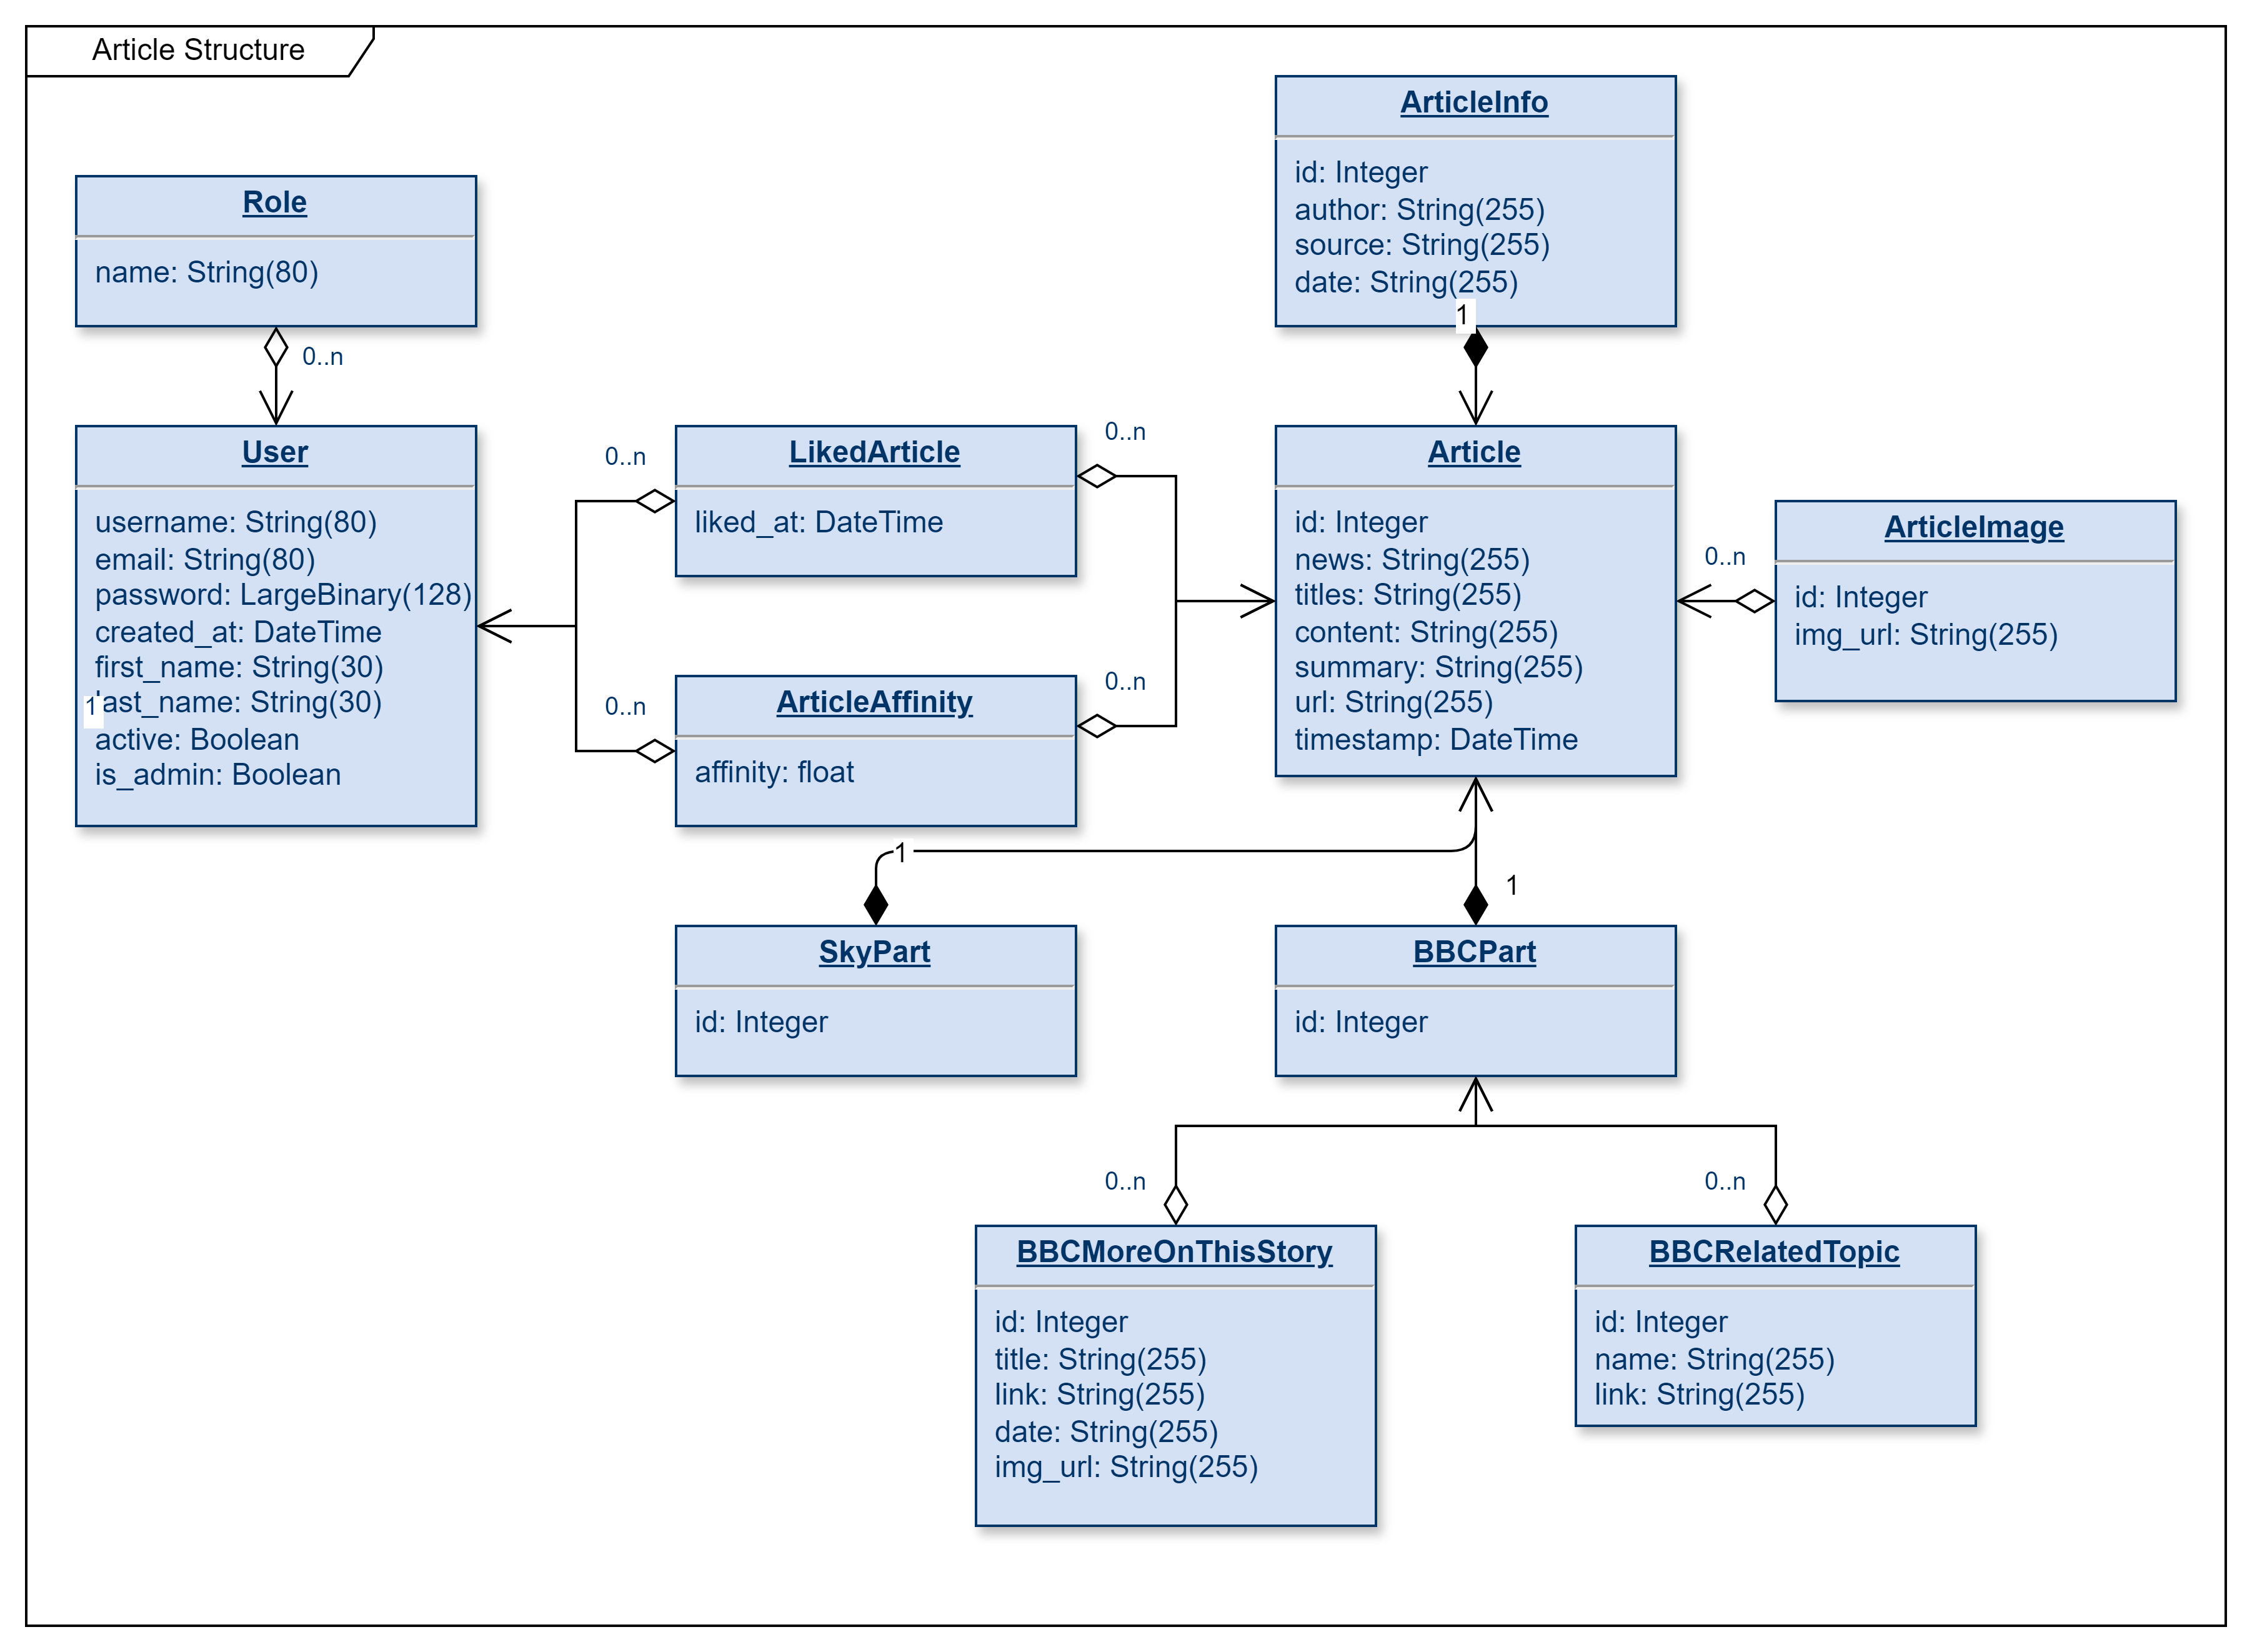
\includegraphics[width=0.9\textwidth]{../Article Structure.png}
    \caption{The database relational structure connecting articles to source-specific parts.}
    \label{fig:article db structure}
\end{figure}

This structure not only streamlines the summarization process but also empowers the application to offer a personalized and intuitive user experience. It mirrors the intricacies of various news formats, thus maintaining the essence of each source while presenting the content in a condensed and accessible format.

\paragraph{Detailed Database Mapping for BBC Articles}

Taking BBC News as a case study, the database is tailored to capture both the homepage's structural elements and the distinctive components that contribute to the unique user experience offered by the BBC News platform.\ref{fig:bbc structure}

\paragraph{Navigation and Homepage Structure}
The database design facilitates the storage of navigational elements and the homepage layout, ensuring users can navigate through the news summary platform as they would on the original BBC site.

\begin{itemize}
    \item \textbf{BBCNavigation Table}: This table preserves the structure of the BBC News navigation bar, recording each navigational item's reference link and title.
    \item \textbf{BBCHomepage Table}: It encapsulates the main content structure of the BBC homepage, including references to regional top stories and various content clusters that define the user's first point of interaction with the news portal.
\end{itemize}

These tables are instrumental in rebuilding the BBC homepage on the summarizer platform, allowing for a direct and familiar experience where users can engage with the content in an environment that mirrors the source website's layout.

\paragraph{Sidebar Specifics}
The BBC's distinctive sidebar, which often contains top stories, featured articles, and the most-read pieces, is re-created using a series of dedicated tables:

\begin{itemize}
    \item \textbf{BBCSidebar Table}: Acts as the anchor for the sidebar, associating each sidebar instance with a unique identifier and a timestamp of when the sidebar was fetched.
    \item \textbf{BBCTopStorySidebar Table}: Categorizes the most prominent stories displayed in the sidebar, complete with titles, links, and publication dates.
    \item \textbf{BBCFeature and MostRead Tables}: These tables classify articles that the BBC features as highlights or identifies as trending across readerships.
\end{itemize}

\begin{figure}[htbp]
    \centering
    \begin{minipage}[t]{0.4\textwidth}
        \raisebox{-\height}{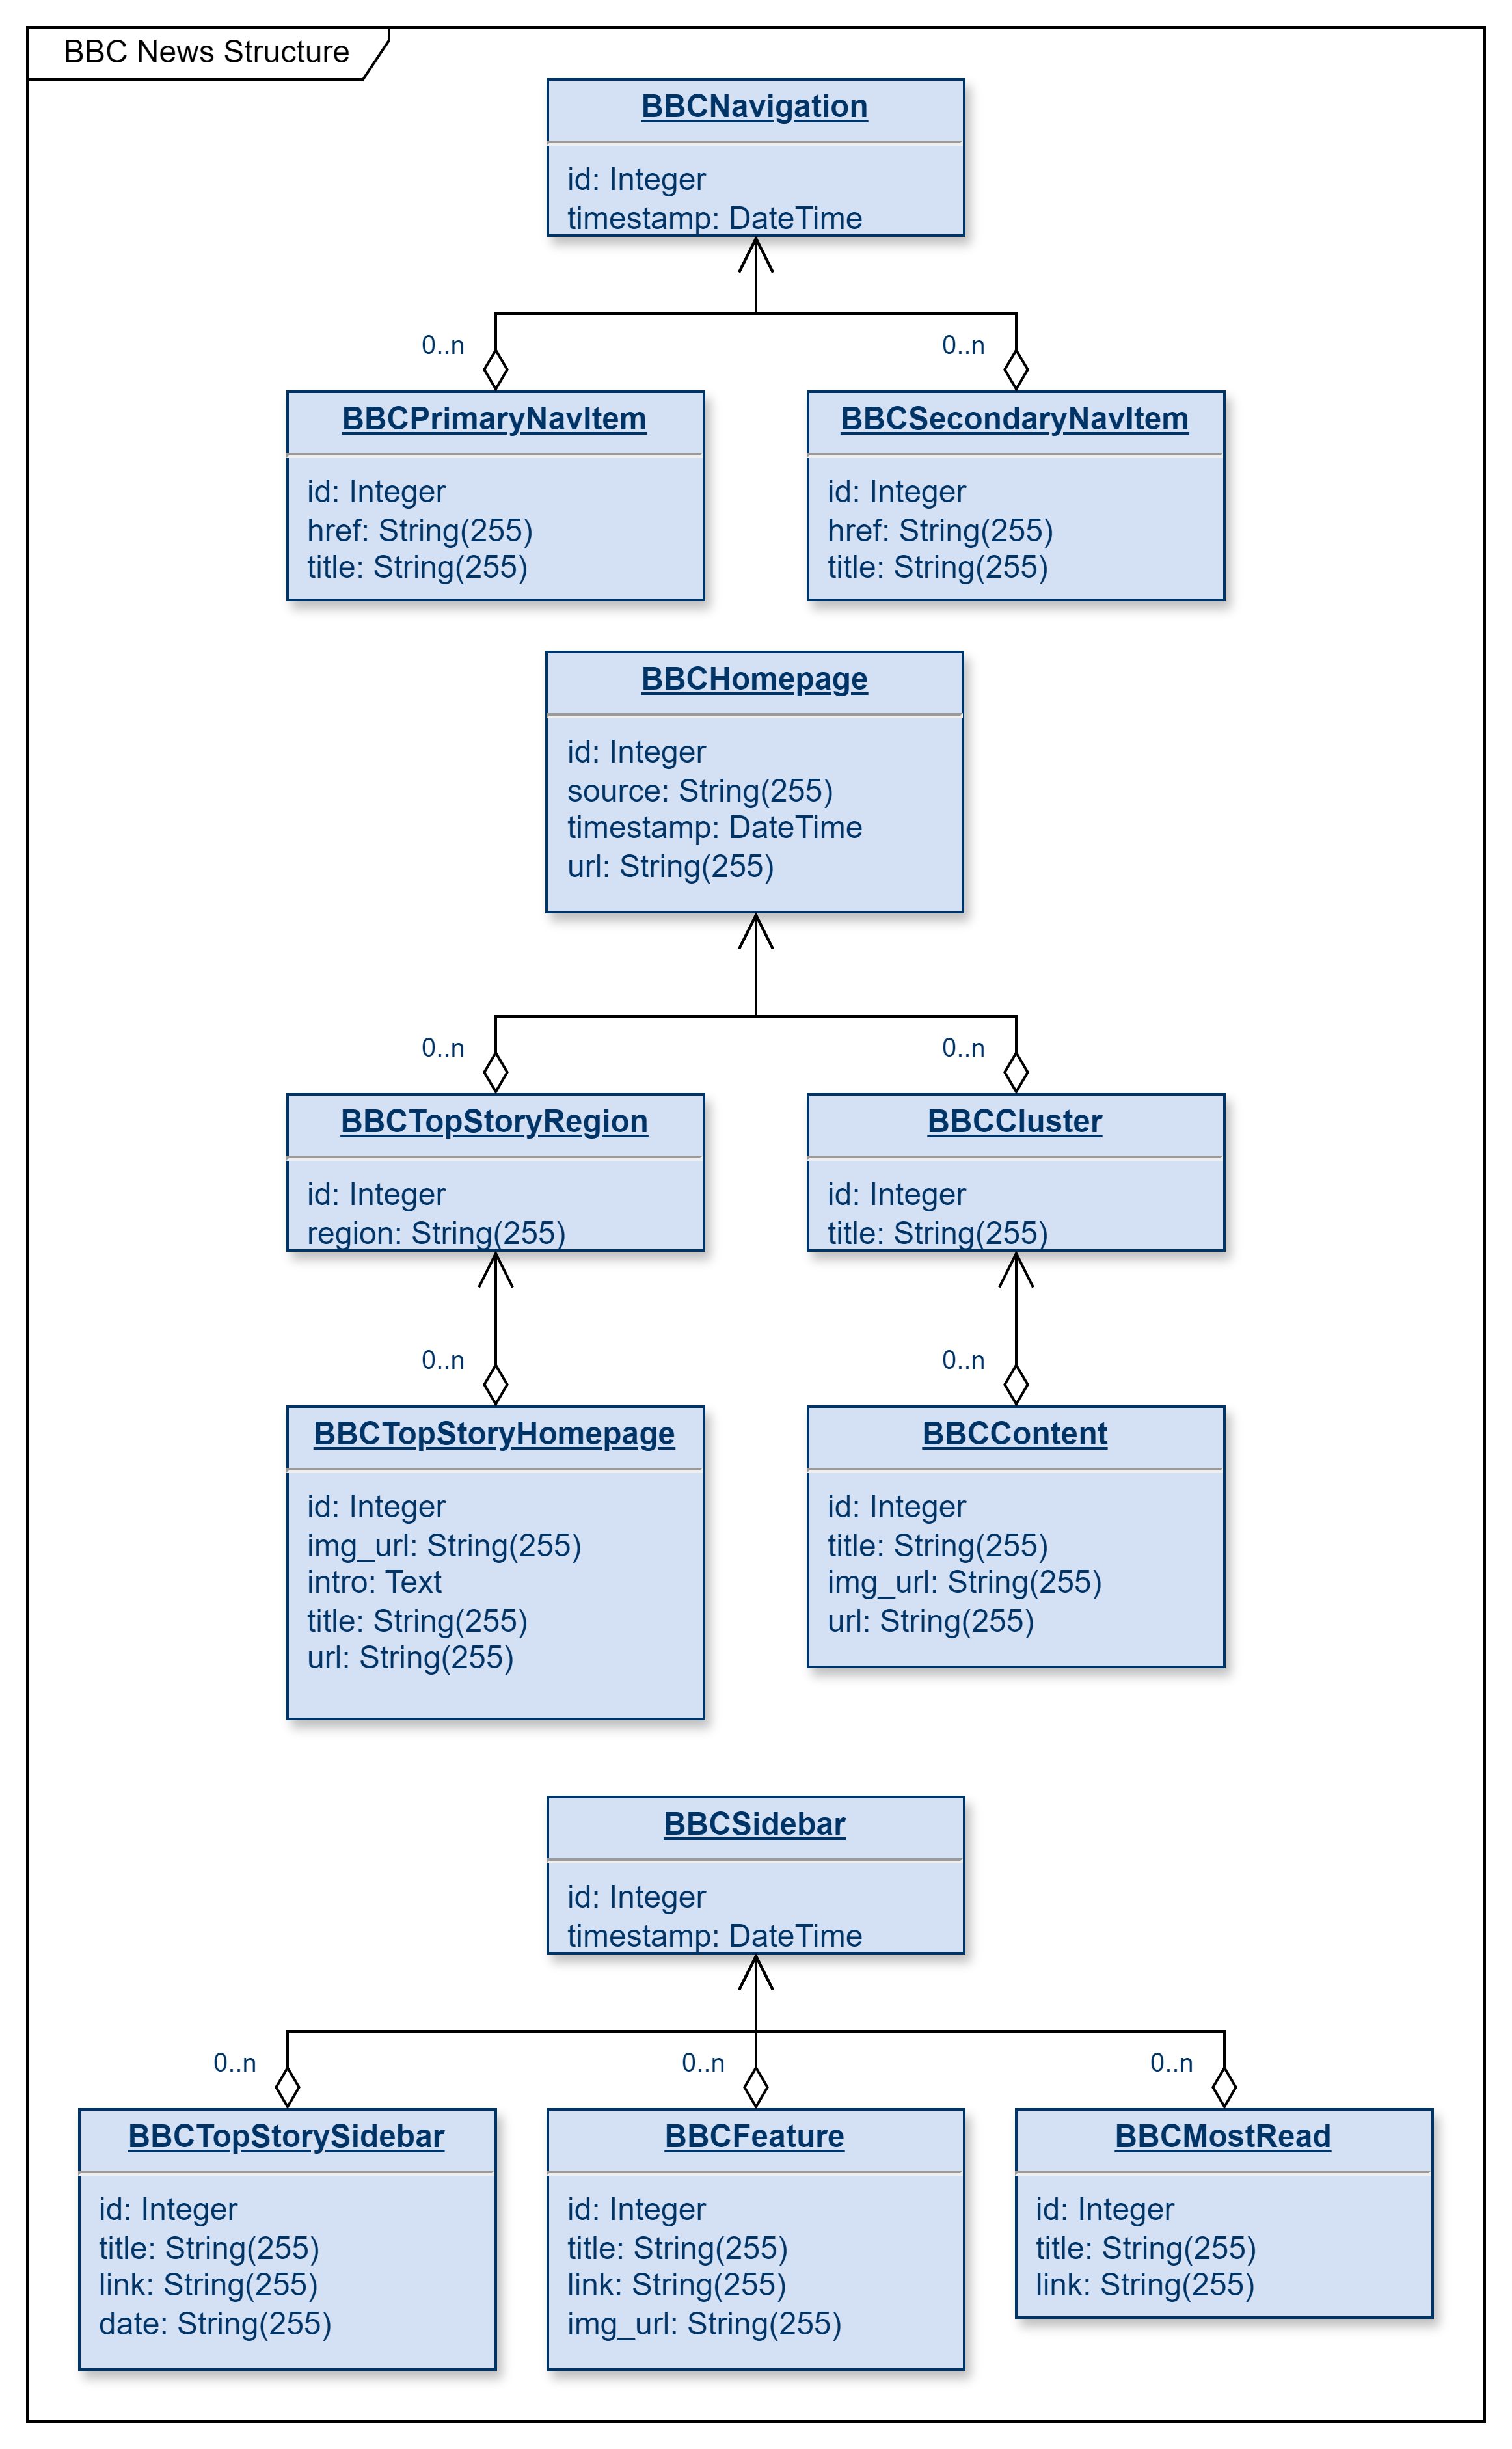
\includegraphics[width=\textwidth]{../BBC Structure.png}}
        \caption{The database relational structure for BBC news}
        \label{fig:bbc structure}
    \end{minipage}
    \hfill
    \begin{minipage}[t]{0.5\textwidth}
        \paragraph{Replicating the BBC User Experience}

        The integration of the homepage and sidebar structures ensures that users of the "Mirror News Summarizer" enjoy a reading experience akin to that provided by the original BBC News website. The database meticulously retains the integrity of the BBC's article presentation style and format.\newline

        This approach of recreating the unique characteristics of news sources within the summarizer platform highlights the project's commitment to a user-centric model. It not only simplifies the reading process but also maintains the editorial and visual cues that BBC News readers are accustomed to, thus bridging the gap between summarized content and the comprehensive news narrative.\newline

        In summary, the detailed database mapping for BBC articles showcases the project's dedication to delivering a seamless and familiar user experience by mimicking the native content structures and presentation styles of varied news sources.\newline
    \end{minipage}
\end{figure}

\newpage
\subsubsection{User Recommendation System}

A critical aspect of the "Mirror News Summarizer" is the personalization of content through a user recommendation system. This intelligent system curates articles that align with individual user interests, utilizing their interaction history with the platform to enhance relevance and engagement. Notably, this feature comes to life upon user authentication, ensuring that personalized content is delivered after login. 

\paragraph{The Recommendation Logic}
The recommendation logic operates in two modes: random selection for new users or similarity-based for users with interaction history. 

\begin{itemize}
    \item \textbf{For New Users:}
    \begin{enumerate}
        \item A set of twelve news articles is randomly selected from the database, ensuring no repetition \\(\textit{get\_random\_news\_from\_db} function).
        \item Articles without a proper title or with the placeholder "No title found" are excluded to maintain content quality.
        \item Each selected article's data, including title, summary, URL, and first image, is compiled into a list for display.
    \end{enumerate}
    
    \item \textbf{For Returning Users:}
    \begin{enumerate}
        \item The system first checks for the existence of liked articles by the user.
        \item If liked articles are present, it employs a \textit{TF-IDF Vectorizer} to transform the textual content of all articles into a mathematical representation.
        \item The similarity between the liked articles and the rest of the corpus is calculated using \textit{cosine similarity}.
        \item Articles are then scored based on their cumulative similarity to the liked articles.
        \item A user-article affinity score is updated or created in the database for later retrieval.
        \item The twelve most similar articles, excluding those already liked, are selected and their data compiled for the user.
    \end{enumerate}
\end{itemize}

\paragraph{Data Structure Utilization}
Throughout this process, the system leverages the previously detailed database structure, interacting with various tables such as:

\begin{itemize}
    \item \textit{Article Table} - Serves as the primary source of content for recommendations.
    \item \textit{LikedArticle Table} - Tracks the articles that have been positively interacted with by the user.
    \item \textit{ArticleAffinity Table} - Stores the affinity score, which is a quantifiable measure of the user's preference towards each article.
    \item \textit{ArticleImage and ArticleInfo Tables} - Provide additional context for each article, enhancing the user experience with visual and metadata elements.
\end{itemize}

The database structure ensures that the recommendation process is both dynamic and responsive, capable of adjusting to user behavior over time. By using real-time data, the "Mirror News Summarizer" delivers personalized content that is not only relevant but also presented in a familiar and engaging manner.

\paragraph{System Efficiency and Scalability}
The recommendation system is optimized for efficiency, minimizing database queries and computational overhead by caching frequently accessed data when appropriate. It's designed to scale with the user base and can accommodate an increasing volume of interactions and content preferences.


\subsubsection{User Interface Design}
Reflecting the project's dedication to a user-centric design philosophy, the "Mirror News Summarizer" employs an interface that is both intuitive and visually engaging. By mirroring the layout of original news sites, it ensures users a seamless reading experience.

\paragraph{Design Philosophy}
Using HTML and CSS, the UI replicates the look and feel of established news outlets. This "mirror style" approach provides familiarity, reducing the learning curve and enhancing user comfort.

\begin{itemize}
    \item Adopts a clean, minimalistic design aligning with modern web standards to minimize distractions and focus on content.
    \item Guarantees a responsive design for a consistent experience across various devices and screen sizes.
    \item Integrates essential features such as user accounts, liking articles, and original article navigation to encourage user interaction.
\end{itemize}

\paragraph{Development Approach}
The UI is developed using the Cookiecutter Flask framework, providing a modular and efficient pathway for incorporating core functionalities.

\begin{itemize}
    \item Combines standard web development practices with Flask's robustness for a stable and scalable user interface.
    \item Incorporates open-source libraries for advanced animations, enriching the UI without overcomplicating the development process.
\end{itemize}

\paragraph{Visual Features and Interactivity}
The summarizer includes several interactive elements that enhance the user experience and make the interface lively:

\begin{itemize}
    \item Features an attractive loading animation, creating a pleasant user experience while waiting for content to be summarized.
    \item Implements functions like liking articles and redirecting to original news in a seamless manner, keeping the interface clean and user-friendly.
\end{itemize}

\paragraph{User Engagement}
The summary loading page is designed to keep the user engaged with an elegant animation, serving as an excellent example of the application's attention to detail in enhancing the user experience.

\begin{figure}[H]
    \centering
    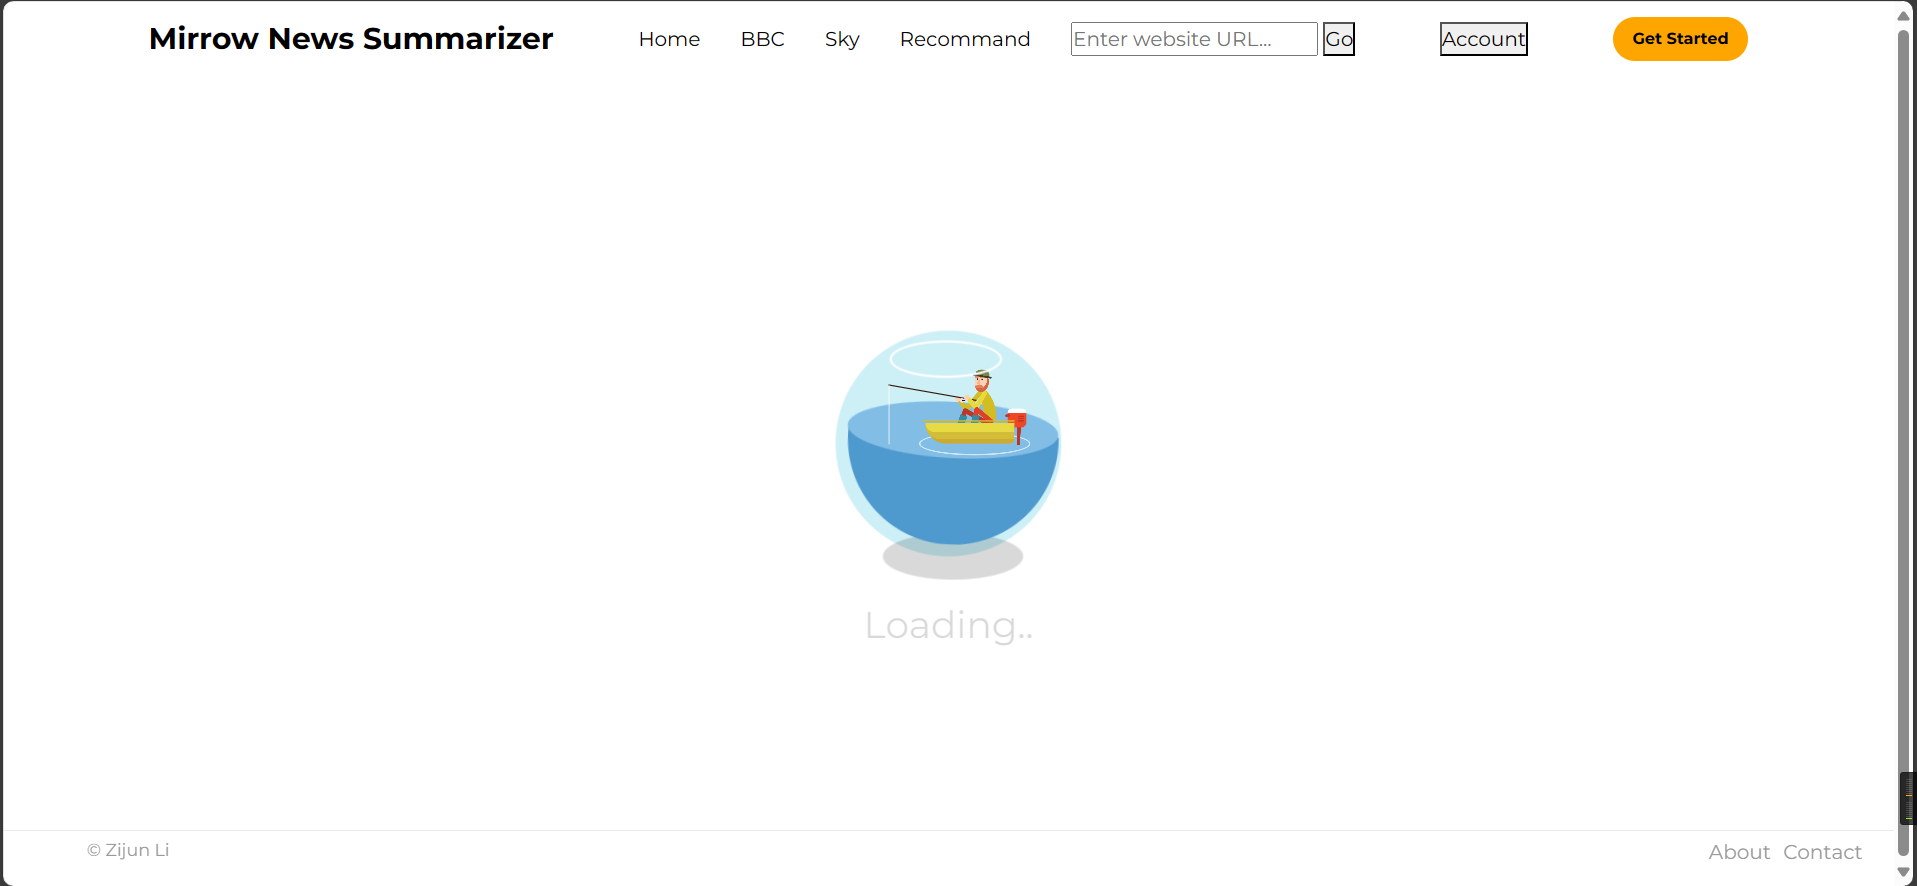
\includegraphics[width=0.8\textwidth]{../loading.png}
    \caption{The loading page animation, indicative of a thoughtful design to enhance user waiting experience.}
\end{figure}

\begin{figure}[H]
    \centering
    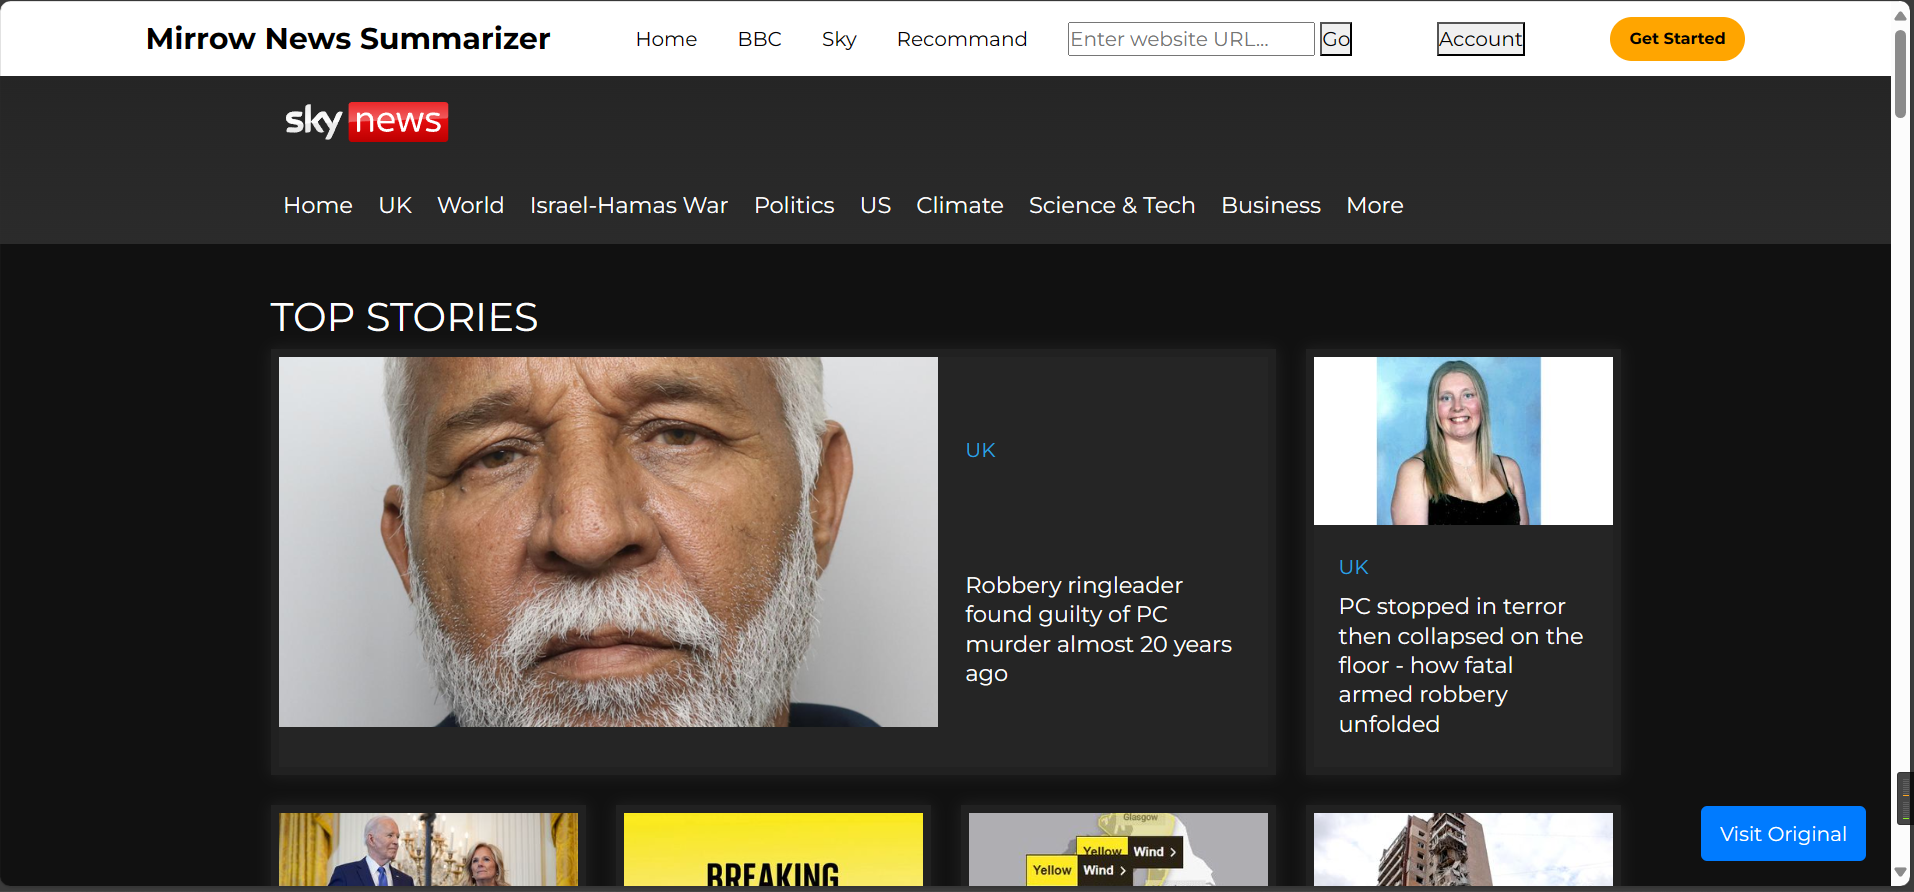
\includegraphics[width=0.8\textwidth]{../Sky news homepage.png}
    \caption{The homepage layout mirrors the familiar design of popular news sources, maintaining consistency and comfort for the user.}
\end{figure}

\begin{figure}[H]
    \centering
    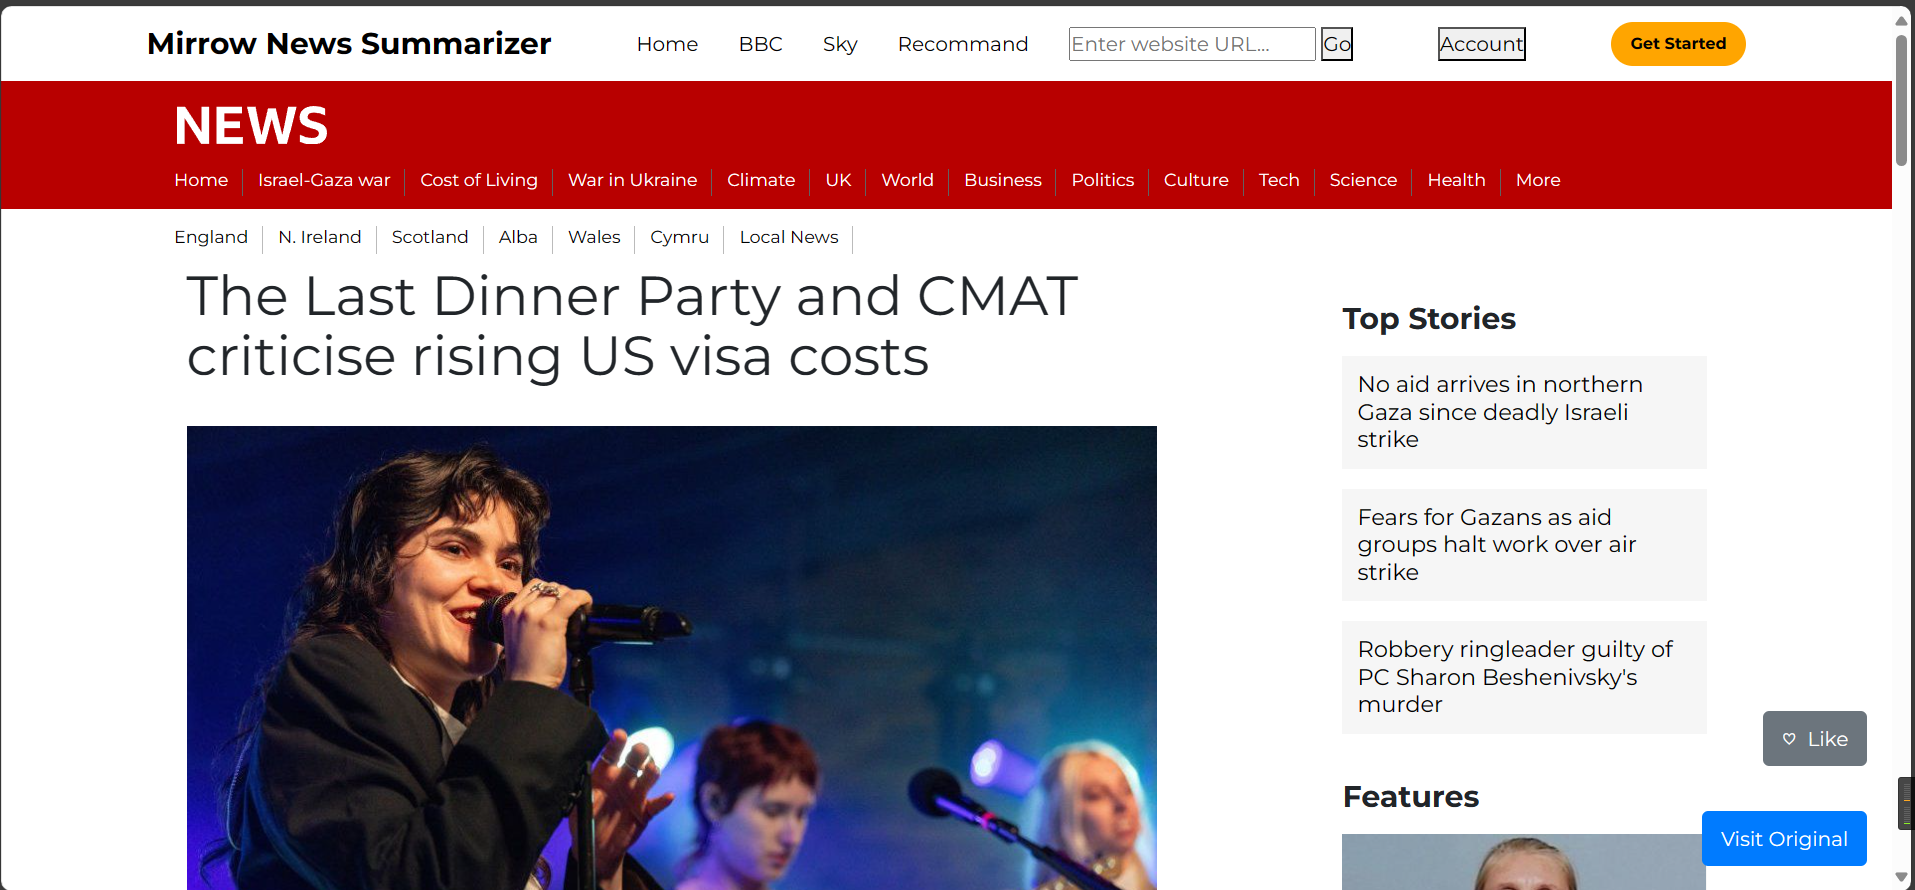
\includegraphics[width=0.8\textwidth]{../BBC news article.png}
    \caption{An article page showing a summary, emulating the style of the source publication for a seamless user experience.}
\end{figure}

\begin{figure}[H]
    \centering
    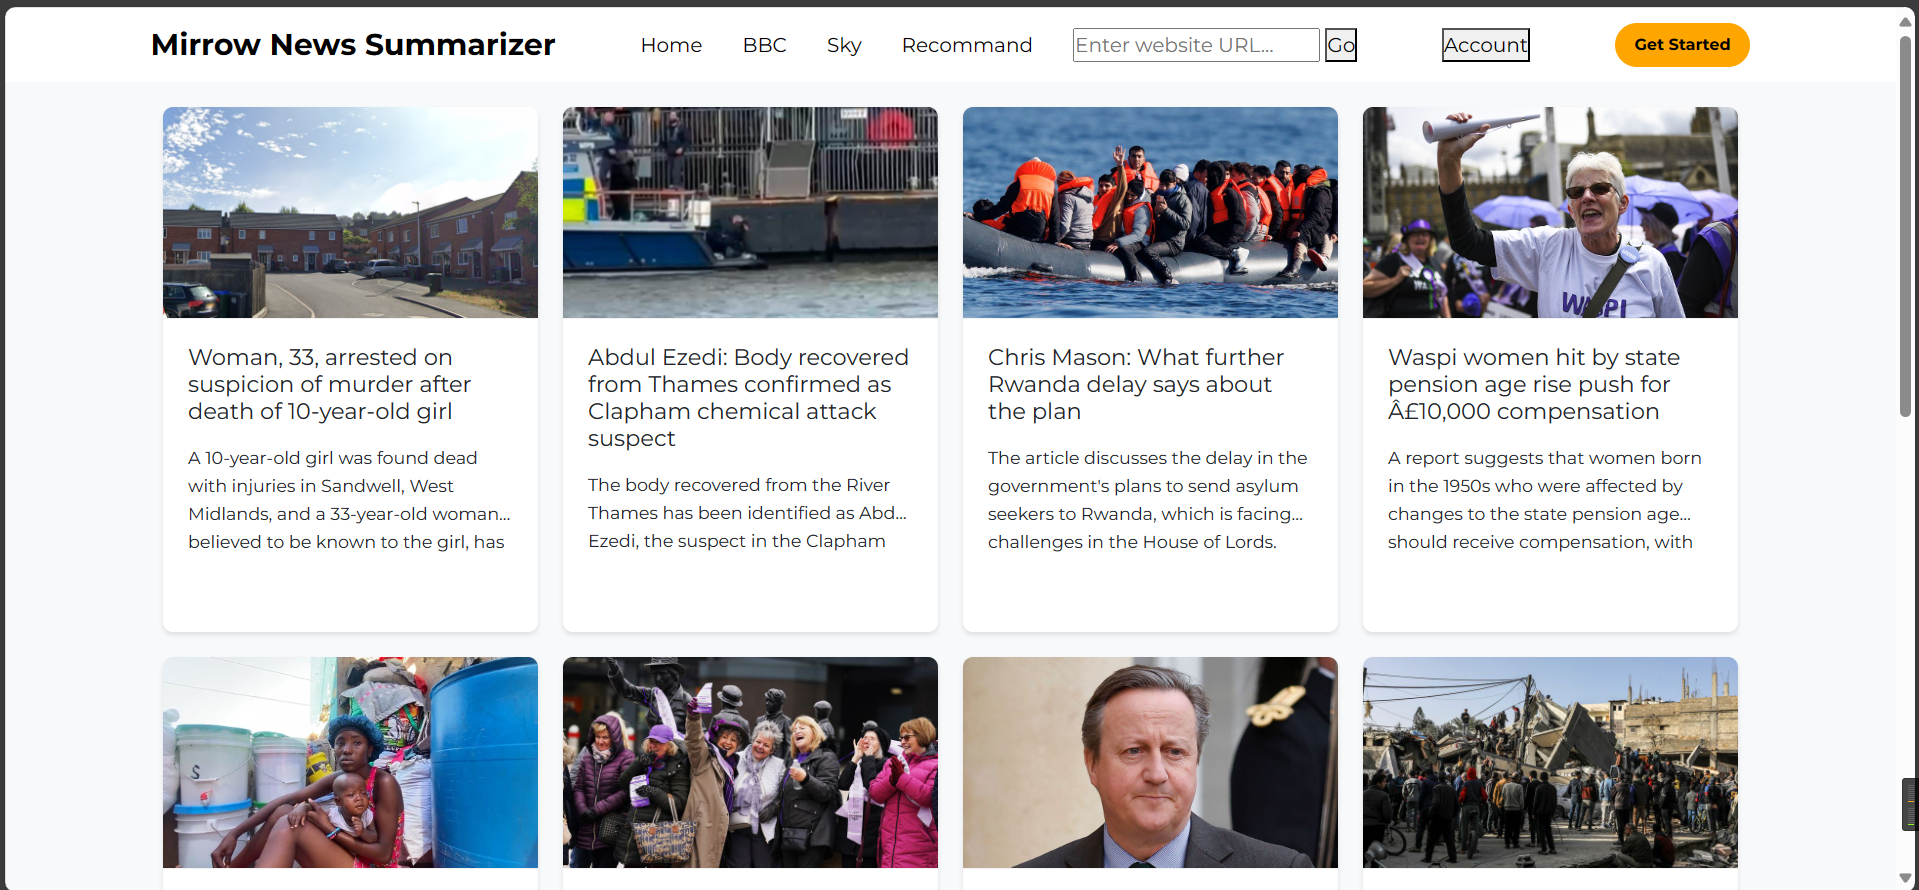
\includegraphics[width=0.8\textwidth]{../recommand.png}
    \caption{The recommendation page, showcasing the system's ability to tailor content to the user's preferences.}
\end{figure}

The design ensures that users are presented with an environment that is not only functional but also visually coherent with the sources they trust, as demonstrated in the homepage and article interface examples.

Moreover, the platform's recommendation system demonstrates a personalized approach to news curation, as seen in the following interface.

In summary, the UI of the "Mirror News Summarizer" is more than a user interface; it's the gateway to a personalized, efficient, and comfortable news consumption experience, crafted with user preferences at the forefront.

\subsection{Design Integration and Framework Selection}

The "Mirror News Summarizer" project's design phase involved a critical decision-making process to select the most suitable framework that would enable efficient integration of frontend, backend, and database components. The focus was on a framework that supports rapid development, scalability, and a user-centric approach to building a responsive UI.

\begin{table}[H]
    \centering
    \begin{tabular}{lccc}
    \hline
    \textbf{Framework} & \textbf{Ease of Setup} & \textbf{Flexibility} & \textbf{Community Support} \\ \hline
    Django\cite{django} & Medium & High & High \\
    Express.js\cite{expressjs} & High & High & High \\
    Ruby on Rails\cite{rubyonrails} & Medium & Medium & High \\
    \textbf{Cookiecutter Flask}\cite{cookiecutterflask} & \textbf{High} & \textbf{High} & \textbf{High} \\ \hline
    \end{tabular}
    \caption{Comparison of Web Application Frameworks}
    \label{tab:framework_comparison}
\end{table}

\paragraph{Framework Evaluation}
In the quest for a suitable framework, a comparative analysis was conducted considering various attributes such as ease of setup, flexibility, and community support. The chosen frameworks for comparison were Django, Express.js, Ruby on Rails, and Cookiecutter Flask. Cookiecutter Flask stood out for its high marks across all categories, as depicted in Table~\ref{tab:framework_comparison}.

\paragraph{Advantages of Cookiecutter Flask}
The rationale for selecting Cookiecutter Flask included several compelling advantages:
\begin{enumerate}
    \item Simplified project scaffolding facilitated a quick start, which was pivotal for adhering to project timelines.
    \item Its unopinionated nature allowed for the bespoke integration of AI summarization and personalization modules.
    \item Flask's lightweight core made it an ideal choice for creating a responsive and dynamic user interface without being bogged down by unnecessary components.
    \item The modular design allowed for integrating functionalities as needed, making the system highly maintainable and scalable.
    \item Robust community support meant that solutions to potential challenges were readily available, reducing the time spent troubleshooting.
\end{enumerate}

\paragraph{Integration Flow}
The UML sequence diagram (Figure~\ref{fig:uml_sequence_diagram}) illustrates the flow of operations from the client's request to the final response delivery. It breaks down the complex interactions into a sequential order, highlighting the Flask application's role as a mediator between the client, database, and external website.

\begin{figure}[H]
    \centering
    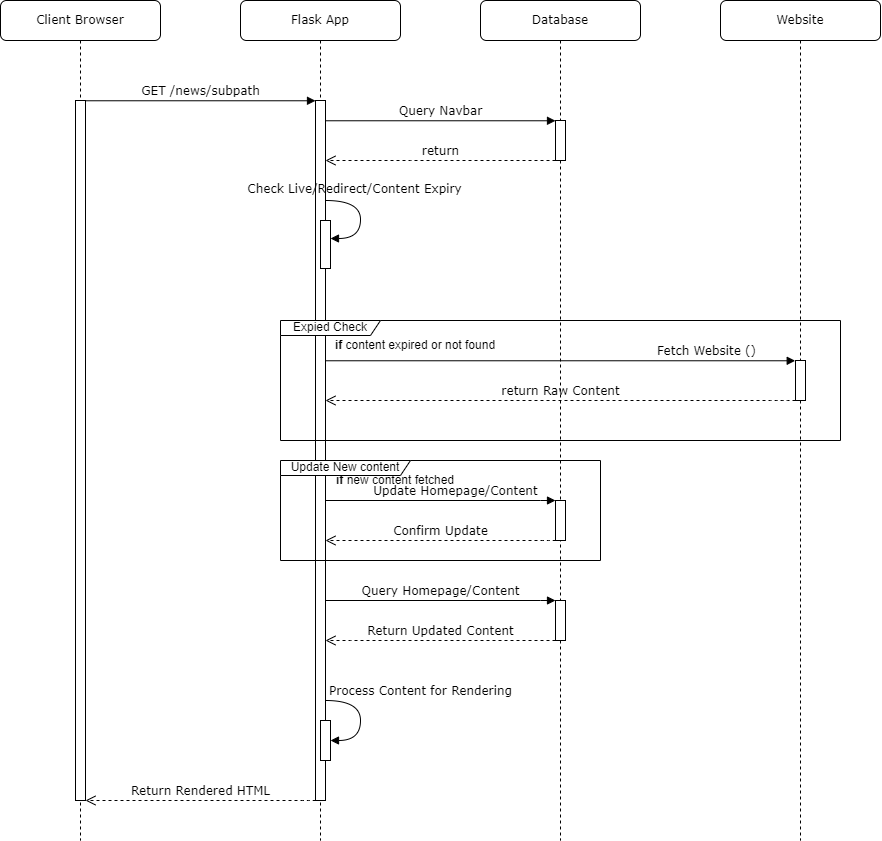
\includegraphics[width=0.95\textwidth]{../UML_app.drawio.png}
    \caption{UML Sequence Diagram illustrating the flow of data in the "Mirror News Summarizer" application.}
    \label{fig:uml_sequence_diagram}
\end{figure}

\paragraph{Sequence of Operations:}
\begin{enumerate}
    \item The Flask application routes incoming requests based on the URL pattern.
    \item It queries the database for navbar items, which are essential for rendering the BBC site's navigation bar.
    \item If the content is marked as live or the request is to redirect, an appropriate response is returned immediately.
    \item For content fetching and updating, the Flask application interacts with the database to check for expired content.
    \item Upon identifying outdated or missing content, it scrapes the BBC website for fresh data.
    \item New content is parsed, processed, and updated in the database.
    \item The updated content is then fetched from the database and sent to the templating engine.
    \item Rendered HTML is returned to the client's browser, providing an updated and responsive view of the requested content.
\end{enumerate}

\paragraph{Usability Focus}
The UI design was iteratively developed to ensure a user-friendly experience. Here, HTML and CSS were used to create layouts that are visually similar to the original news websites, fostering a familiar environment for users. While the animations were borrowed from \href{https://github.com/Lavender-z/demo/tree/master}{open-source libraries}, they were carefully selected and integrated to complement the overall design aesthetics and provide visual feedback during content loading.

\paragraph{Application Features}
The project boasts essential features such as user authentication, article bookmarking, and redirection to original news articles. Additionally, the user experience is enhanced by the thoughtfully designed loading animations, which provide a smooth transition while the summarization content is being prepared for display.

In conclusion, the application's architecture is a testament to the efficiency of Cookiecutter Flask in crafting a cohesive system where AI-driven backend services are seamlessly connected to a user-focused frontend, leading to an application that is both robust and delightful to use.

\section{Project Management}

The development and management of the "Mirror News Summarizer" project were underpinned by a combination of agile methodologies, version control, and a modular approach to software design. This section discusses the project management strategies that were employed, emphasizing the structure and development aspects such as frontend design, database architecture, backend integration, and server deployment.

\subsection{Agile Methodology}

The project was managed using agile principles, which facilitated flexibility and iterative development. Bi-weekly sprints were established to prioritize tasks, allowing for rapid adjustments based on testing feedback and unforeseen challenges. This iterative approach enabled continuous improvement of the application, ensuring that features like the news summarizer, user interface, and personalized content delivery were developed and refined progressively.

\subsection{Version Control}

Git was adopted for version control, with the repository hosted on GitLab. This allowed for effective tracking of changes, collaboration, and feature branching. The use of feature branches ensured that the development of new functionalities, such as parser integration or UI enhancements, could be done without disrupting the main application. This strategy also facilitated the implementation of code reviews, enhancing the quality and maintainability of the codebase.

\subsection{Modular Software Design}

The software architecture of the "Mirror News Summarizer" was designed with modularity in mind. This approach allowed for the separation of concerns among different components of the application:

\begin{itemize}
    \item \textbf{Frontend Web Design}: HTML and CSS were utilized to create a responsive and intuitive user interface. The design focused on mirroring the layout of original news websites to provide a familiar experience for users. Modular CSS files and HTML templates enabled a consistent look and feel across different parts of the application.
    \item \textbf{Database Architecture}: The project used a relational database to store user data, article summaries, and source content. The database schema was designed to support efficient data retrieval and updates, crucial for the personalized content delivery mechanism.
    \item \textbf{Backend Integration}: Flask, a Python web framework, facilitated the backend integration, connecting the frontend with the database and external news sources. The backend was responsible for handling user requests, executing the summarization process, and serving personalized news feeds.
    \item \textbf{Server Deployment}: The application was deployed on an Amazon EC2 instance, ensuring scalability and accessibility. The deployment process involved setting up a Linux environment, configuring the web server.
\end{itemize}

\section{Results}

\subsection{Outcome}

The \textit{Mirror News Summarizer} project has yielded significant achievements in streamlining news consumption and enhancing user interaction. The project's results are categorized based on the fulfillment of key functional requirements. The deployed version of the platform can be accessed at \href{http://35.178.153.233:5000/}{Mirror News Summarizer}(\href{http://35.178.153.233:5000/}{http://35.178.153.233:5000/}) for a hands-on experience with its features and functionalities.

\begin{itemize}
    \item \textbf{Summarization Functionality}: The core feature of the platform, AI-driven summarization, is functioning as intended. It has been validated through extensive user testing to ensure that summaries are both concise and contextually complete.\ref{fig:result_summary}
    
    \begin{figure}[H]
        \centering
        \includegraphics[width=0.8\textwidth]{../result_summary.png}
        \caption{Comparison between an original article and its AI-generated summary.}
        \label{fig:result_summary}
    \end{figure}

    \newpage
    \item \textbf{Personalization Accuracy}: Leveraging machine learning algorithms, the system has successfully tailored news feeds to match individual user preferences, leading to higher levels of user satisfaction and engagement. This is evidenced by the positive user feedback and the increased interaction with the summarizer's recommendations.\ref{fig:ui_design}\ref{fig:user_retention}

    \begin{figure}[H]
        \centering
        \includegraphics[width=0.7\textwidth]{../UI Design.png}
        \caption{The user interface of the "Mirror News Summarizer" showcasing its clean and intuitive layout.}
        \label{fig:ui_design}
    \end{figure}

    \begin{figure}[H]
        \centering
        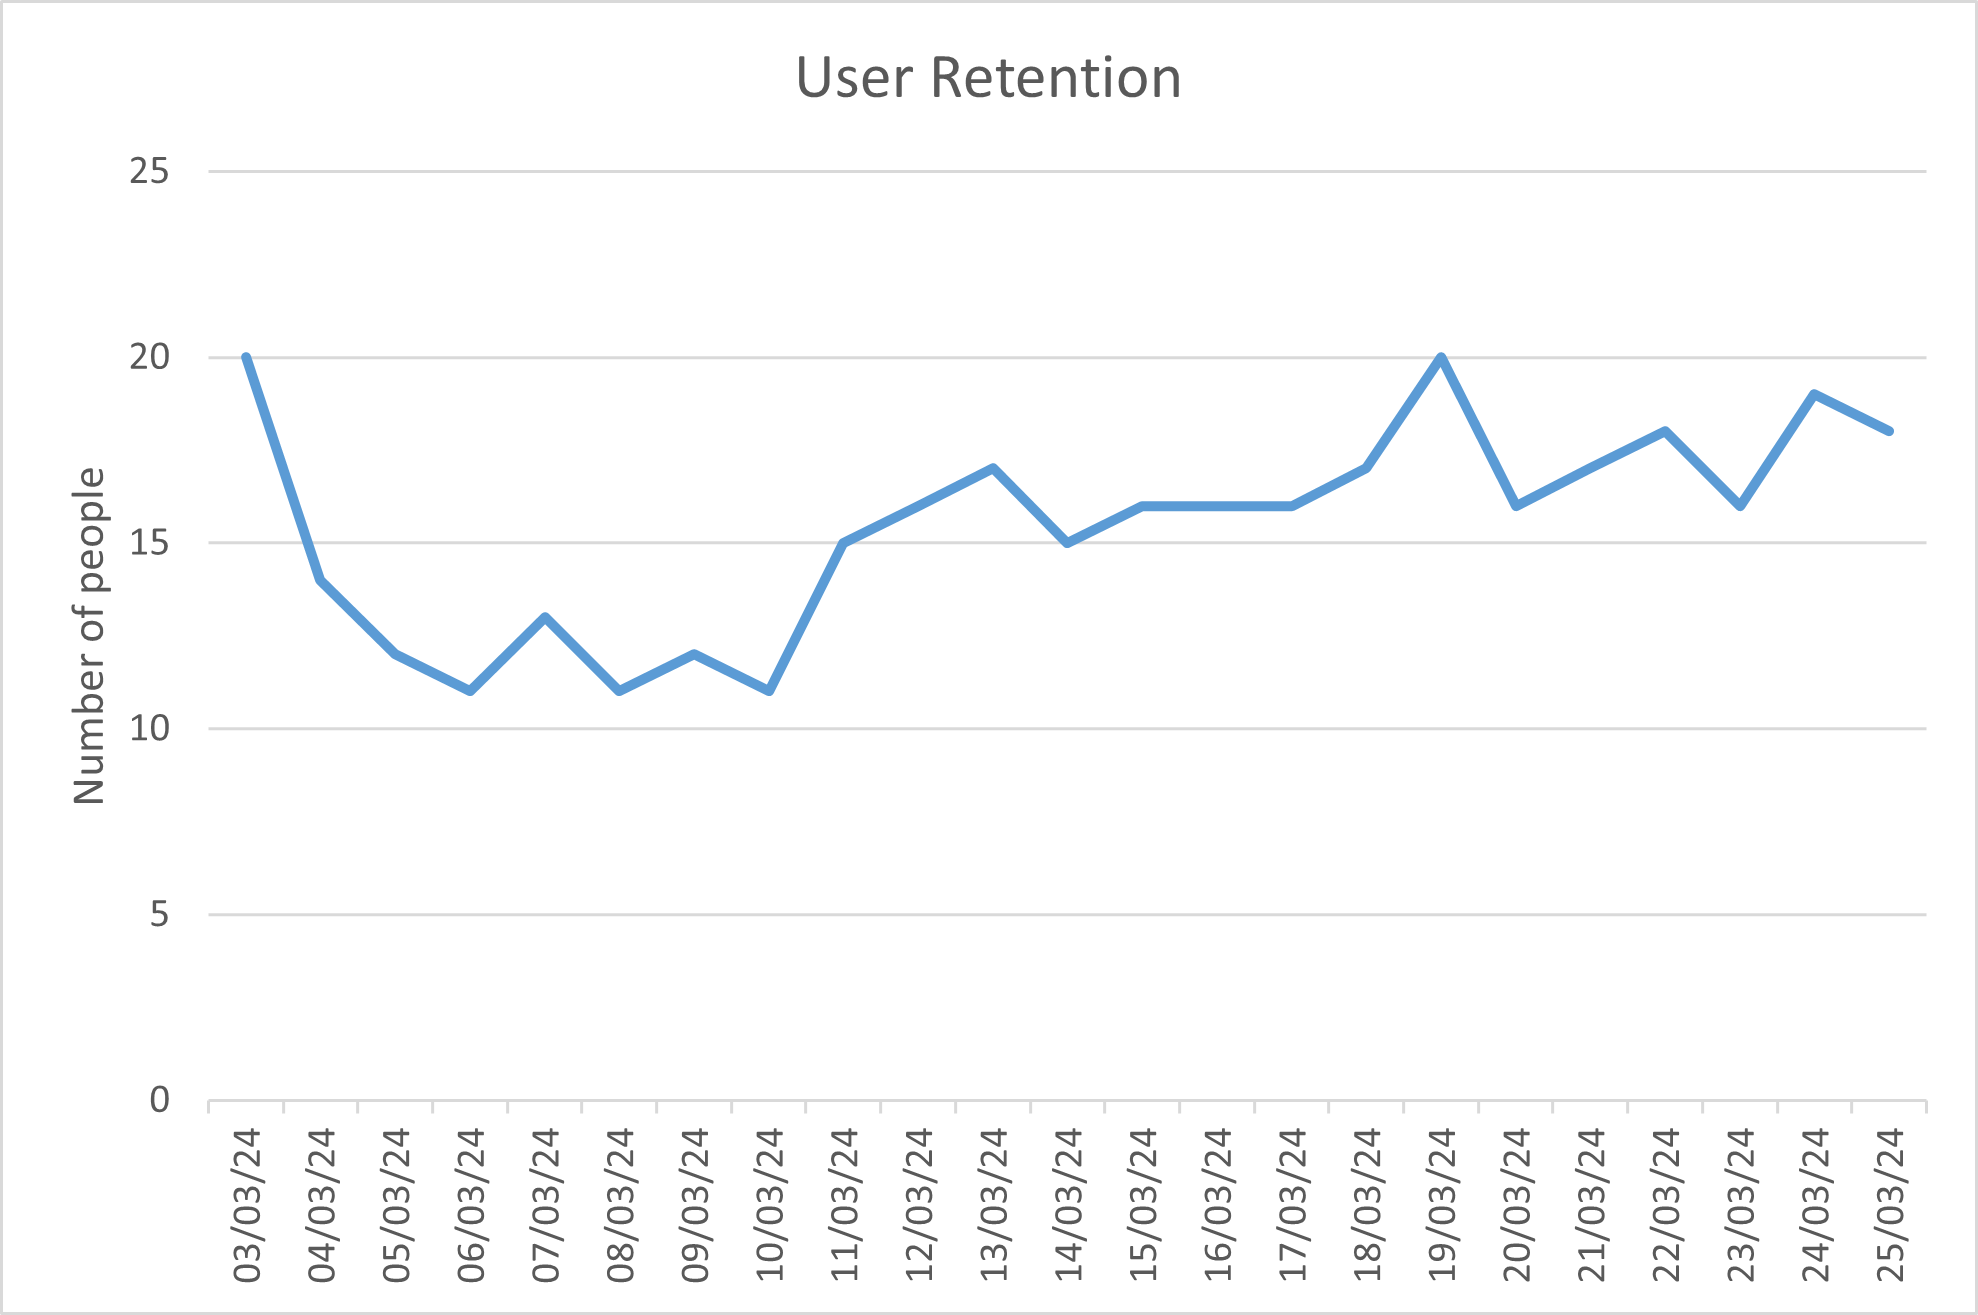
\includegraphics[width=0.7\textwidth]{../user retention.png}
        \caption{User retention rates before and after the introduction of personalized news feeds.}
        \label{fig:user_retention}
    \end{figure}
    
    \item \textbf{Backend-Frontend Integration}: The seamless integration between backend services and the frontend presentation has been confirmed through real-time system monitoring, ensuring up-to-date content delivery without performance hiccups.\ref{fig:integration}
    
    \begin{figure}[H]
        \centering
        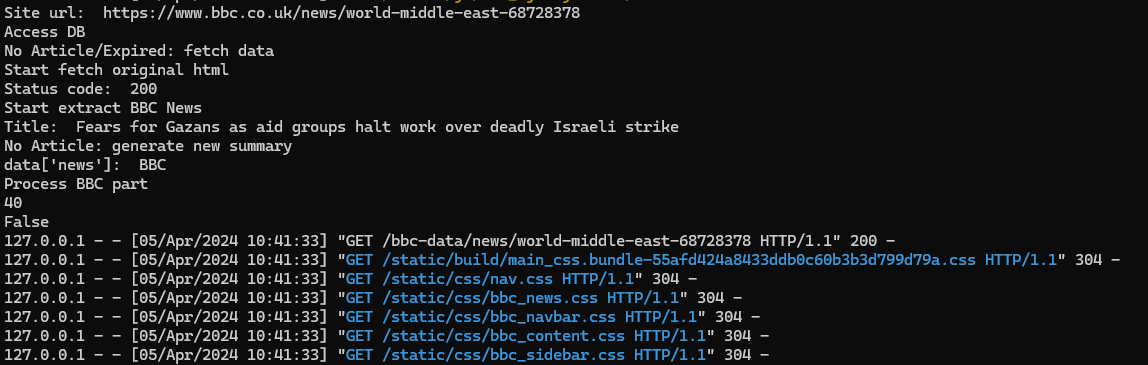
\includegraphics[width=0.7\textwidth]{../integration.png}
        \caption{real-time system monitoring data.}
        \label{fig:integration}
    \end{figure}

\end{itemize}

\subsection{Functional Requirement Fulfillment}

The project has met its functional requirements as evidenced by the outcomes:

\begin{itemize}
    \item \textbf{Real-time Summarization}: Users receive immediate article summaries upon request, with average processing times well within the target range(around 8 seconds).
    \item \textbf{Adaptive Content Curation}: The system dynamically adjusts the news feed based on user interactions, with a marked improvement in content relevance reported by users.
    \item \textbf{Responsive User Interface}: Cross-platform usability tests confirm that the interface adapts effectively to different devices, maintaining a consistent user experience.
\end{itemize}

\subsection{Highlights of User Experience}

Feedback channels established during the project have offered a transparent view of the user experience, revealing high satisfaction with both the content and the delivery system:

\begin{itemize}
    \item Users report a notable reduction in the time spent sifting through news, thanks to efficient summarization.
    \item The "Like" feature and direct links to original articles have seen substantial use, indicating the effectiveness of these engagement tools.
    
    \item The interactive loading animation has been mentioned frequently in user testimonials, emphasizing the importance of engaging UI elements.
    
\end{itemize}

These reflections on user experience underscore the platform's capacity to not only present news in a digestible format but also to foster an interactive and user-friendly environment.

\subsection{Contributions}

One of the significant contributions of the "Mirror News Summarizer" project is the development and open-sourcing of the News Fetcher tool, a comprehensive software solution for parsing and extracting structured data from BBC and Sky News websites. This tool, available on GitHub at \url{https://github.com/VergilOP/News-Fetcher}, represents a pivotal resource for researchers, journalists, and anyone interested in conducting media analysis or aggregating news content for various applications.

\paragraph{Key Contributions of News Fetcher}
News Fetcher simplifies the process of accessing and utilizing news data by offering:
\begin{itemize}
    \item Automated parsing capabilities for BBC and Sky News, enabling efficient extraction of headlines, lead paragraphs, and detailed article content.
    \item Modular design for easy adaptation and expansion, allowing the integration of additional news sources or content types.
    \item Open-source availability, encouraging community collaboration, and innovation in the field of digital media analysis.
\end{itemize}

\paragraph{Impact on the Project}
The News Fetcher project significantly enhances the "Mirror News Summarizer" by providing a reliable and scalable backend tool for news data acquisition. It ensures that the summarizer has access to timely and relevant content, which is crucial for maintaining the accuracy and relevance of the summarizations provided to users. Moreover, by sharing this tool with the broader community, the project contributes to the collective effort to make digital news more accessible and analyzable.

\paragraph{Acknowledgments and Disclaimer}
The project team extends its gratitude to BBC and Sky News for maintaining comprehensive and accessible news platforms, which serve as the foundation for this contribution. While News Fetcher is designed for educational and research purposes, users are reminded to adhere to the terms of service of the respective news outlets when utilizing the software.

\section{Evaluation}

\subsection{Testing Procedures}

The "Mirror News Summarizer" underwent a comprehensive evaluation to ensure its robustness, functionality, and user satisfaction. Utilizing the Flask framework's built-in `flask test` command facilitated a multifaceted testing approach:

\begin{itemize}
    \item \textbf{Automated Testing}: Unit and integration tests were implemented to verify the accuracy and interoperability of system components, ensuring the application's core functionalities performed as expected.
    
    \item \textbf{Performance and Security Testing}: Simulated scenarios tested the application's performance under load, and security assessments identified vulnerabilities, reinforcing the system's defenses against potential cyber threats.
    
    \item \textbf{Usability Testing}: Feedback from potential users was invaluable in refining the user interface and overall experience, guiding iterative improvements.
\end{itemize}

A noteworthy result of the `flask test` execution was the successful passage of all tests, underscoring the application's readiness. However, the process also highlighted areas for future enhancement, particularly regarding code coverage and the resolution of deprecation warnings.

Here's a concise version of the test execution output using the `verbatim` environment to maintain the structure and clarity of the original output:

\noindent\begin{Verbatim}[fontsize=\scriptsize]
PS C:\mirror-news-summarizer\> flask test
================================================= test session starts =================================================
platform win32 -- Python 3.11.3, pytest-7.4.4, pluggy-1.3.0 -- C:\Users\XXX\AppData\Local\Programs\Python\Python311\python.exe
cachedir: .pytest_cache
rootdir: \mirror-news-summarizer\
plugins: anyio-3.6.2, Faker-21.0.0, hydra-core-1.3.2, cov-4.1.0
collected 30 items

tests/test_database.py::TestCRUDMixin::test_create PASSED                                                        [  3%]
tests/test_database.py::TestCRUDMixin::test_create_save PASSED                                                   [  6%]
tests/test_database.py::TestCRUDMixin::test_delete_with_commit PASSED                                            [ 10%]
tests/test_database.py::TestCRUDMixin::test_delete_without_commit_cannot_access PASSED                           [ 13%]
tests/test_database.py::TestCRUDMixin::test_update[True-bar] PASSED                                              [ 16%]
tests/test_database.py::TestCRUDMixin::test_update[False-foo] PASSED                                             [ 20%]
tests/test_database.py::TestPkModel::test_get_by_id_wrong_type PASSED                                            [ 23%]
tests/test_forms.py::TestRegisterForm::test_validate_user_already_registered PASSED                              [ 26%]
tests/test_forms.py::TestRegisterForm::test_validate_email_already_registered PASSED                             [ 30%]
tests/test_forms.py::TestRegisterForm::test_validate_success PASSED                                              [ 33%]
tests/test_forms.py::TestLoginForm::test_validate_success PASSED                                                 [ 36%]
tests/test_forms.py::TestLoginForm::test_validate_unknown_username PASSED                                        [ 40%]
tests/test_forms.py::TestLoginForm::test_validate_invalid_password PASSED                                        [ 43%]
tests/test_forms.py::TestLoginForm::test_validate_inactive_user PASSED                                           [ 46%]
tests/test_functional.py::TestLoggingIn::test_can_log_in_returns_200 PASSED                                      [ 50%]
tests/test_functional.py::TestLoggingIn::test_sees_alert_on_log_out PASSED                                       [ 53%]
tests/test_functional.py::TestLoggingIn::test_sees_error_message_if_password_is_incorrect PASSED                 [ 56%]
tests/test_functional.py::TestLoggingIn::test_sees_error_message_if_username_doesnt_exist PASSED                 [ 60%]
tests/test_functional.py::TestRegistering::test_can_register PASSED                                              [ 63%]
tests/test_functional.py::TestRegistering::test_sees_error_message_if_passwords_dont_match PASSED                [ 66%]
tests/test_functional.py::TestRegistering::test_sees_error_message_if_user_already_registered PASSED             [ 70%]
tests/test_models.py::TestUser::test_get_by_id PASSED                                                            [ 73%]
tests/test_models.py::TestUser::test_created_at_defaults_to_datetime PASSED                                      [ 76%]
tests/test_models.py::TestUser::test_password_is_nullable PASSED                                                 [ 80%]
tests/test_models.py::TestUser::test_factory PASSED                                                              [ 83%]
tests/test_models.py::TestUser::test_check_password PASSED                                                       [ 86%]
tests/test_models.py::TestUser::test_full_name PASSED                                                            [ 90%]
tests/test_models.py::TestUser::test_roles PASSED                                                                [ 93%]
tests/test_models.py::TestUser::test_roles_repr PASSED                                                           [ 96%]
tests/test_models.py::TestUser::test_user_repr PASSED                                                            [100%]

---------- coverage: platform win32, python 3.11.3-final-0 -----------
Name                                                           Stmts   Miss  Cover
----------------------------------------------------------------------------------
mirror_news_summarizer\__init__.py                                 0      0   100%
...
----------------------------------------------------------------------------------
TOTAL                                                           1782   1661     7%

=========================================== 30 passed, 35 warnings in 1.52s ===========================================
\end{Verbatim}

This testing phase not only validated the "Mirror News Summarizer"'s functionality but also laid a groundwork for ongoing enhancements. Future work will focus on addressing identified warnings and improving code coverage to further solidify the application's quality and user experience.

\subsection{User Acceptance Testing (UAT) Execution}

The User Acceptance Testing (UAT) for the "Mirror News Summarizer" was meticulously designed to validate the project against end-user requirements and expectations. A multi-step UAT process was devised, capturing the full spectrum of user interactions and ensuring that the platform's deliverables were not only functional but also resonated with the user experience.

\paragraph{Preparation and Planning}
Prior to UAT commencement, we delineated the scope and objectives in a detailed UAT plan. This involved:
\begin{itemize}
    \item Defining the key features of the summarizer to be tested, such as real-time summarization, personalization of news feeds, and the user engagement elements.
    \item Drafting clear acceptance criteria for each feature to serve as benchmarks for successful testing outcomes.
    \item Selecting a diverse group of end-users for participation, encompassing students, educators, professionals, and news enthusiasts to reflect our broad user base.
    \item Preparing realistic test data that represented typical user interactions with news articles.
\end{itemize}

\paragraph{Test Scenario Development}
We constructed comprehensive test scenarios that mirrored real-world usage:
\begin{itemize}
    \item Scenarios covered typical user journeys, including signing up, configuring personal preferences, using the summarization feature, and engaging with personalized content.
    \item Test cases within each scenario were designed to validate not only the functionality but also the usability and responsiveness of the system.
\end{itemize}

\paragraph{UAT Execution}
During UAT execution:
\begin{itemize}
    \item Participants engaged with the system, executing the designed test cases. Test sessions were monitored to capture any deviations from expected outcomes.
    \item The testing was facilitated by a simple-to-use interface for reporting issues and providing feedback in real-time, which was crucial for capturing the user experience.
\end{itemize}

\paragraph{Feedback Analysis and Refinements}
Following UAT execution:
\begin{itemize}
    \item Feedback was consolidated, categorized, and analyzed. Issues were prioritized based on their impact on the user experience and the platform's operational objectives.
    \item Where necessary, immediate refinements were implemented, and additional rounds of UAT were conducted to ensure all critical issues were addressed satisfactorily.
\end{itemize}

\paragraph{Business Objectives Confirmation}
The UAT was concluded with a review against the initial business objectives to ensure alignment and satisfaction:
\begin{itemize}
    \item Each feature was vetted to confirm it met the outlined acceptance criteria.
    \item User feedback was evaluated to ensure that the platform not only performed as expected but also delivered a user experience that met or exceeded expectations.
\end{itemize}

The rigorous UAT cycle confirmed that the "Mirror News Summarizer" successfully met the fundamental requirements essential for enhancing the news reading experience. The platform's ability to provide succinct summaries and curated content was validated, confirming its readiness for deployment.

% Insert the previously provided table of UAT feedback

\begin{table}[H]
\centering
\begin{tabular}{|p{1cm}|p{4cm}|p{10cm}|}
\hline
\textbf{User} & \textbf{Role} & \textbf{Feedback} \\
\hline
U01 & Zijun(Developer)\ref{fig:persona-zijun} & ``I tested the system for bugs and was pleased with its performance. The backend integration seems solid and reliable.'' \\
\hline
U02 & Brian(Student)\ref{fig:persona-brian} & ``I loved how the personalized feed worked. It showed me content related to my studies and interests without me having to look for it.'' \\
\hline
U03 & Binhao(News Enthusiast)\ref{fig:persona-binghao} & ``Being able to like articles and come back to them later is very useful. The personal touches are noticeable and appreciated.'' \\
\hline
U04 & Renzhi (Professional)\ref{fig:persona-renzhi} & ``The loading animation is a smart touch. It's a small detail, but it shows that thought has been put into the user experience.'' \\
\hline
U05 & Liqun(Educator)\ref{fig:persona-liqun} & ``As an educator, having a tool that distills information quickly is invaluable. The summaries are well-crafted, highlighting key points effectively.'' \\
\hline
U06 & Bin(Researcher)\ref{fig:persona-bin} & ``The absence of ads and unnecessary clutter makes for a focused reading experience. It’s what sets this platform apart from others.'' \\
\hline
U07 & Sabour(College Student)\ref{fig:persona-sabour} & ``The UI is responsive and well-organized, making it easy to find and read articles on my phone.'' \\
\hline
\end{tabular}
\caption{User Acceptance Testing Feedback}
\label{table:uat_feedback}
\end{table}

\subsection{Evaluation Summary}

The feedback from UAT, alongside the results from the earlier testing phases, suggests that the "Mirror News Summarizer" is well-received and meets the needs of a diverse user base. The positive reception of the summarization accuracy and the UI design indicates that the application fulfills its goal of simplifying news consumption. The constructive comments also provide a roadmap for future enhancements and underline the importance of continuous user engagement in the development process.

\newpage

\section{Conclusion}

The "Mirror News Summarizer" project has demonstrated significant strides in addressing the challenges of digital news consumption. By leveraging artificial intelligence for content summarization and providing a user-friendly interface, the project has successfully reduced information overload and enhanced the user engagement. This section concludes the report by reflecting on the achievements and envisioning the future trajectory of the platform.

\subsection{Achievements}

The project has met and, in some instances, exceeded its primary objectives. Key achievements include:

\begin{itemize}
    \item \textbf{Efficient News Summarization}: The AI summarization technology has been validated to deliver concise summaries without compromising content integrity, vastly improving the efficiency of news consumption.
    \item \textbf{Personalization}: By tailoring the content to user preferences, the platform has significantly increased user engagement and satisfaction, confirming the efficacy of the personalization algorithms.
    \item \textbf{User Experience}: The minimalist design, intuitive navigation, and absence of distracting elements have provided a superior user experience, as evidenced by the positive feedback during UAT.
    \item \textbf{Technical Robustness}: The seamless integration of backend and frontend components has ensured real-time updates and system reliability, which is crucial for maintaining user trust.
\end{itemize}

\subsection{Future Prospects}

Looking forward, the "Mirror News Summarizer" is poised for further development and growth. Potential future enhancements include:

\begin{itemize}
    \item \textbf{Expansion of News Sources}: Integrating a broader spectrum of news outlets to cater to a more diverse user base.
    \item \textbf{Advanced AI Models}: Continuously improving the summarization and personalization algorithms for greater accuracy and user relevance.
    \item \textbf{Multilingual Support}: Implementing multilingual capabilities to serve a global audience and foster inclusivity.
    \item \textbf{Community Features}: Exploring the addition of social features, allowing users to discuss and share news within the platform.
    \item \textbf{Voice Integration}: Providing voice-enabled functionalities for accessibility and convenience.
\end{itemize}

The envisioned advancements aim to solidify the "Mirror News Summarizer" as a leader in digital news consumption, addressing the evolving needs of users in an increasingly interconnected world.

\subsection{Final Reflections}

The "Mirror News Summarizer" stands as a testament to the potential of combining AI with user-centric design to enhance the way we consume news. It underscores the importance of adaptability and user-focused innovation in the ever-changing landscape of digital media. As we look to the future, the project serves as a foundation for continuous improvement, setting the stage for a new era of personalized, efficient, and engaging news consumption.

\newpage

\printbibliography

\section*{Personas of user}

\begin{figure}[H]
    \centering
    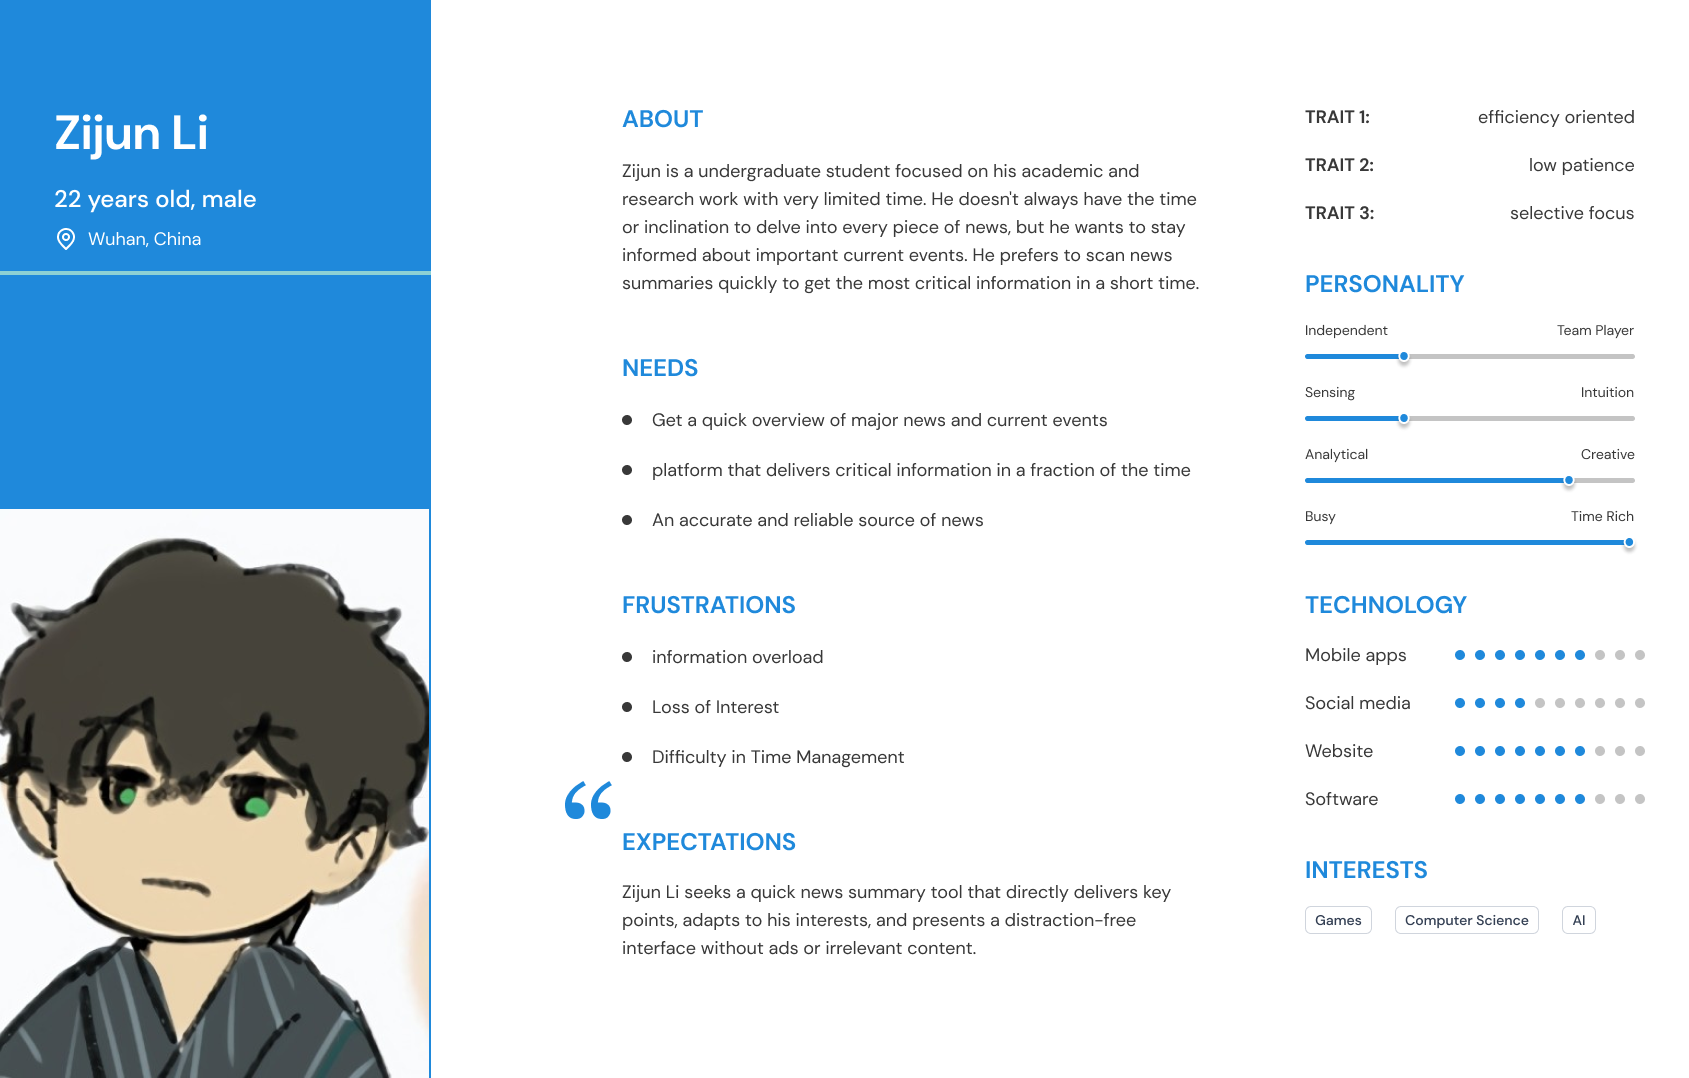
\includegraphics[width=\textwidth]{../persona zijun.png}
    \caption{Persona: Zijun}
    \label{fig:persona-zijun}
\end{figure}

\begin{figure}[H]
    \centering
    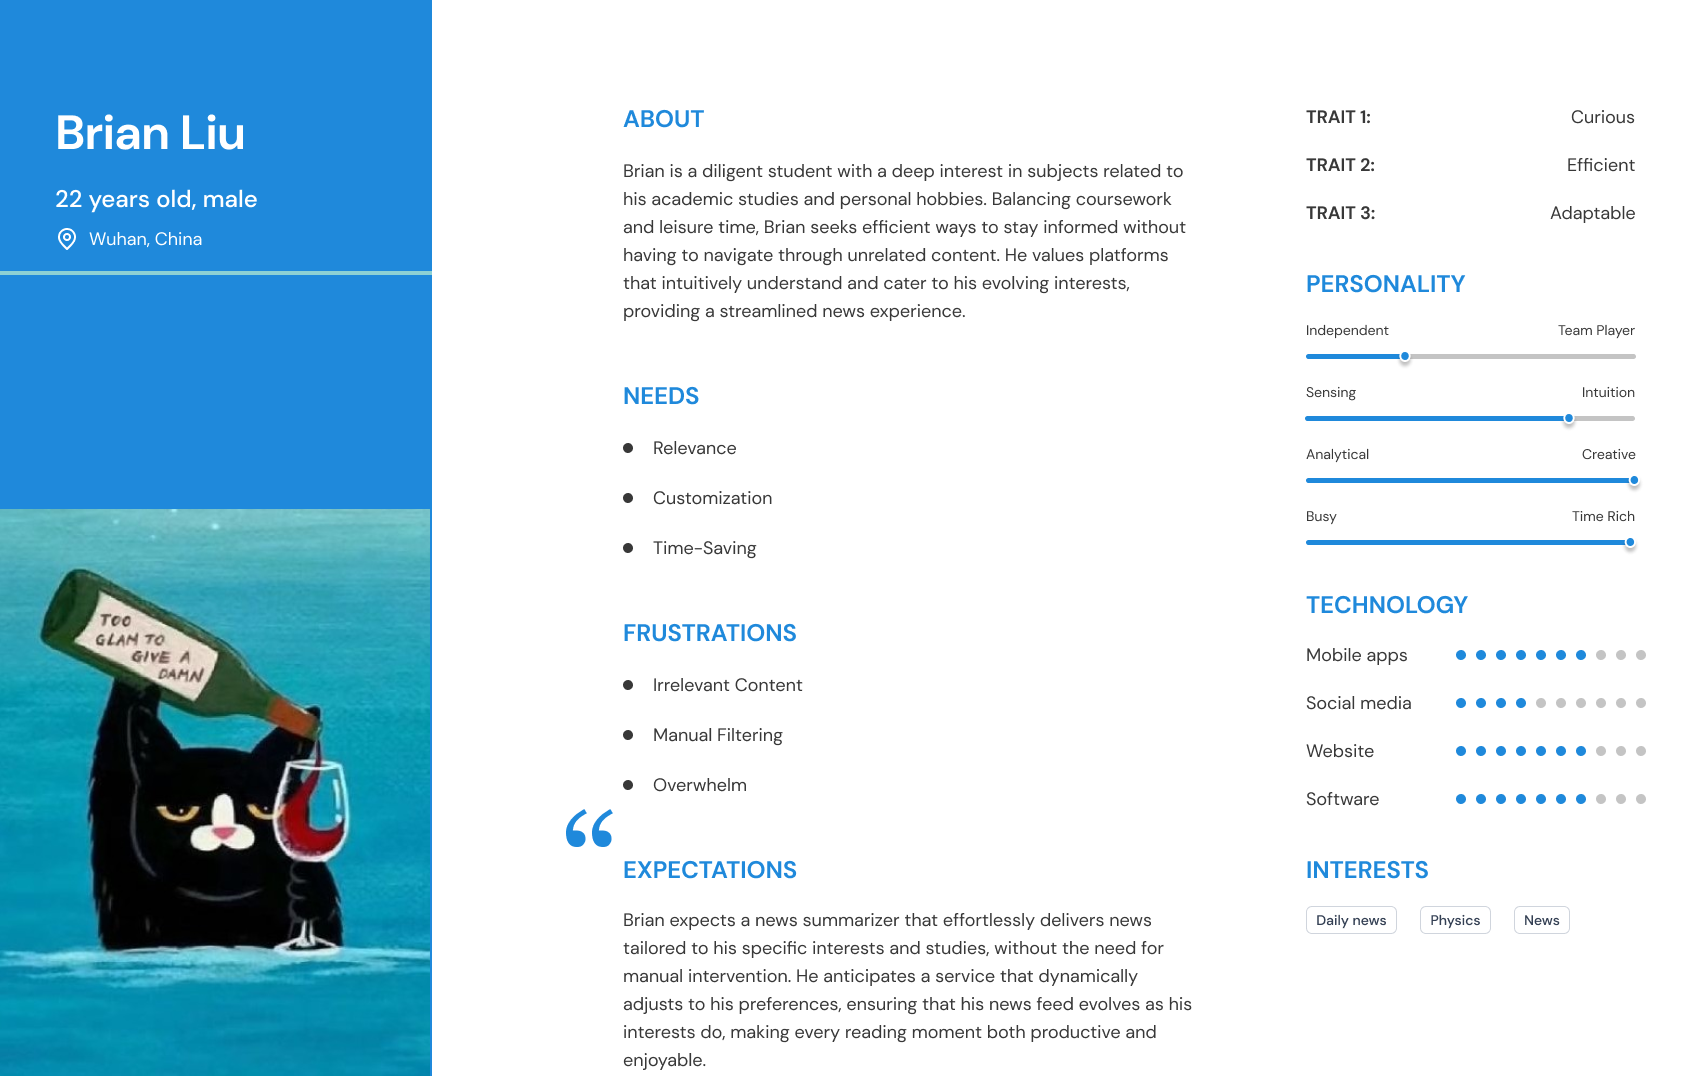
\includegraphics[width=\textwidth]{../persona brian.png}
    \caption{Persona: Brian}
    \label{fig:persona-brian}
\end{figure}

\begin{figure}[H]
    \centering
    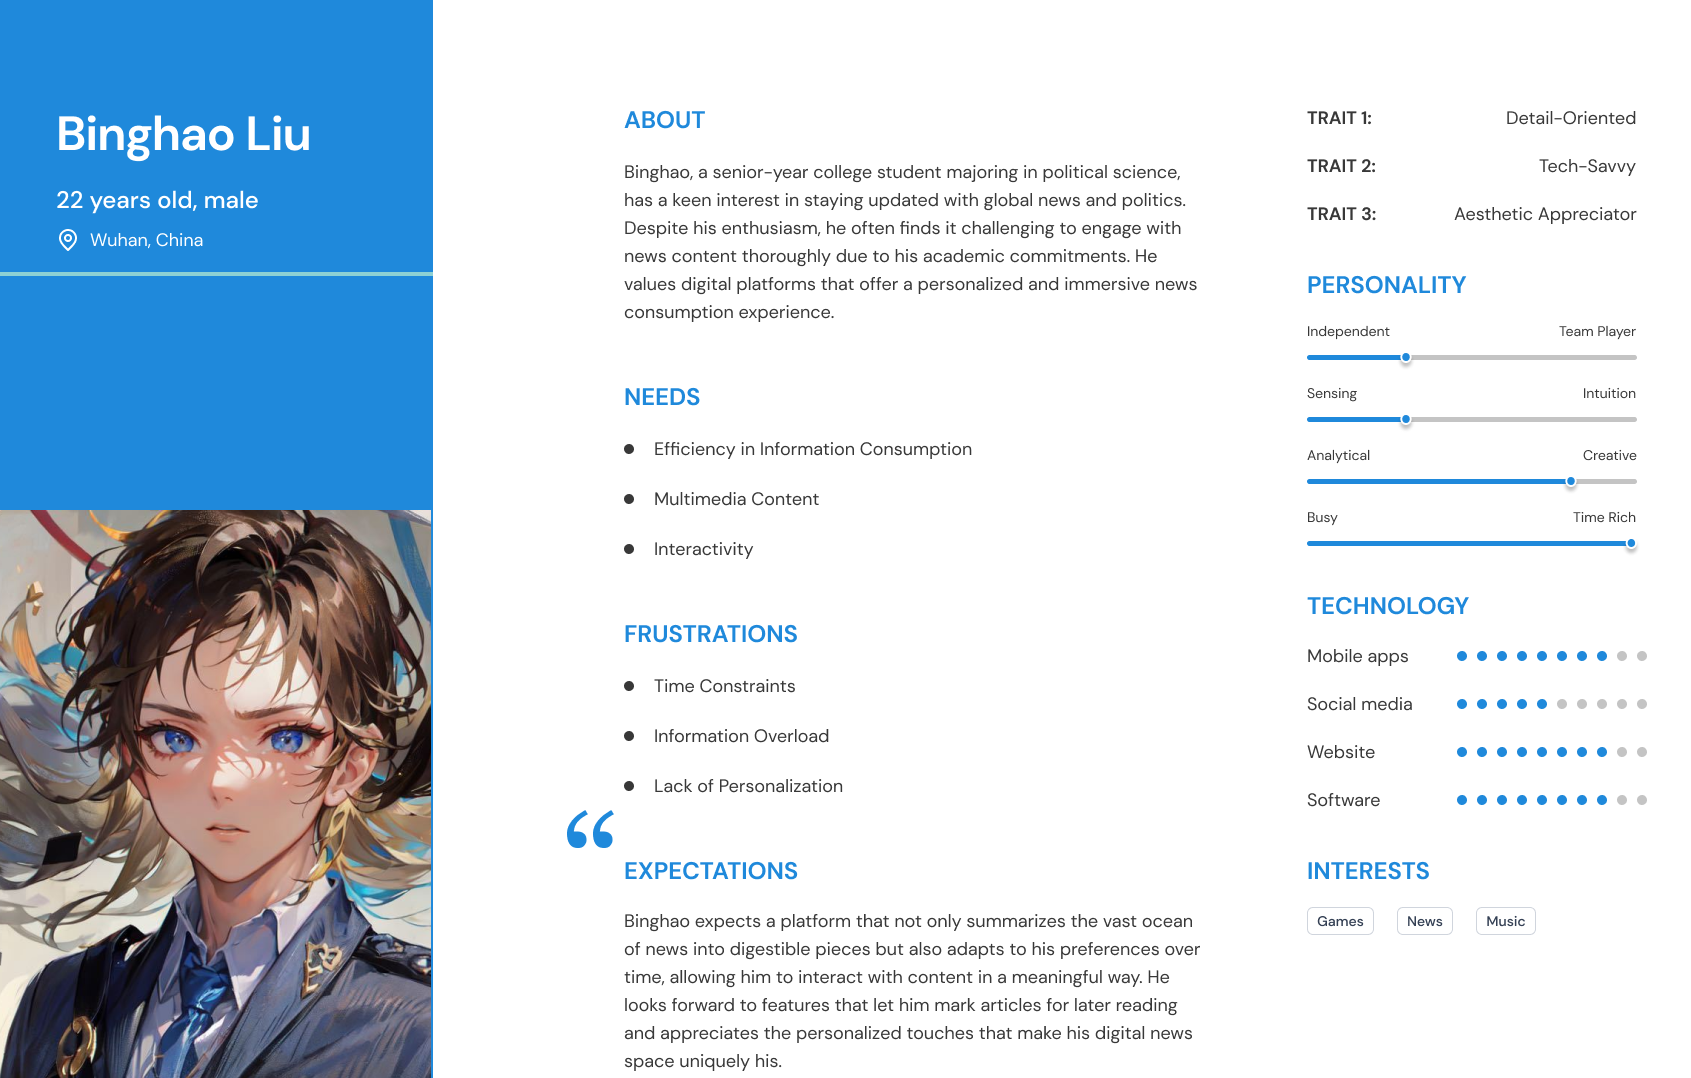
\includegraphics[width=\textwidth]{../persona binghao.png}
    \caption{Persona: Binghao}
    \label{fig:persona-binghao}
\end{figure}

\begin{figure}[H]
    \centering
    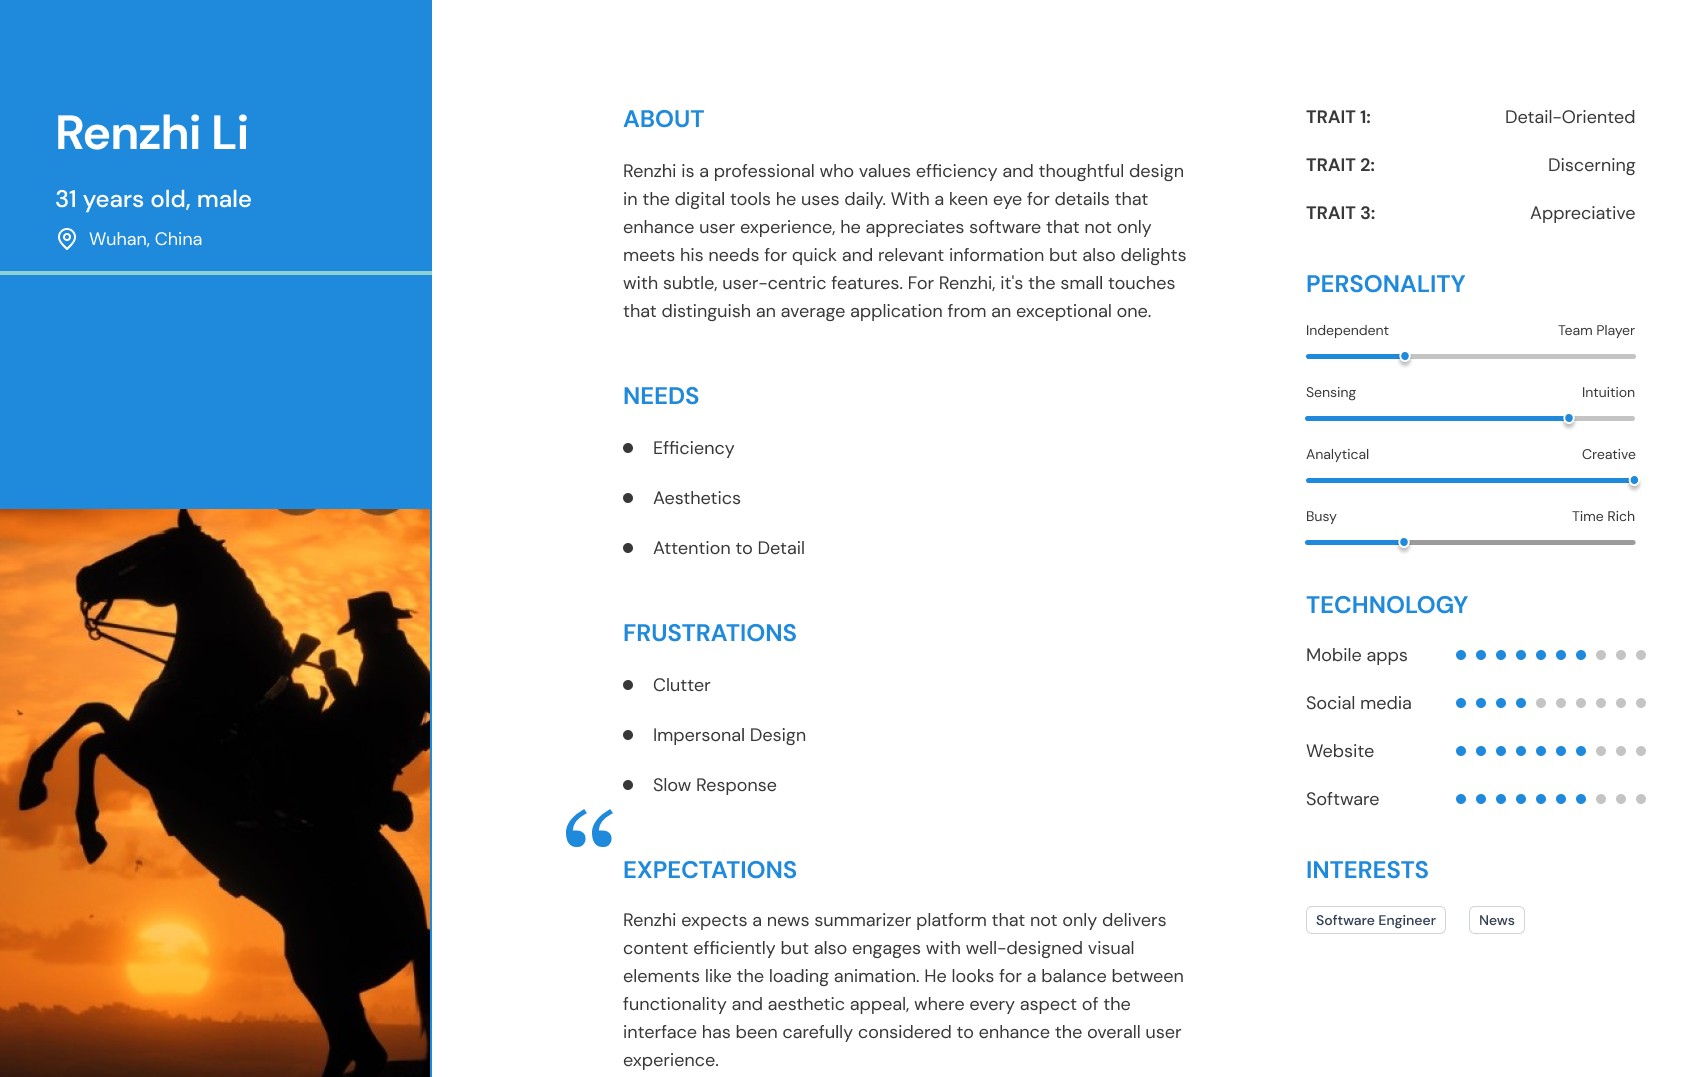
\includegraphics[width=\textwidth]{../persona renzhi.png}
    \caption{Persona: Renzhi}
    \label{fig:persona-renzhi}
\end{figure}

\begin{figure}[H]
    \centering
    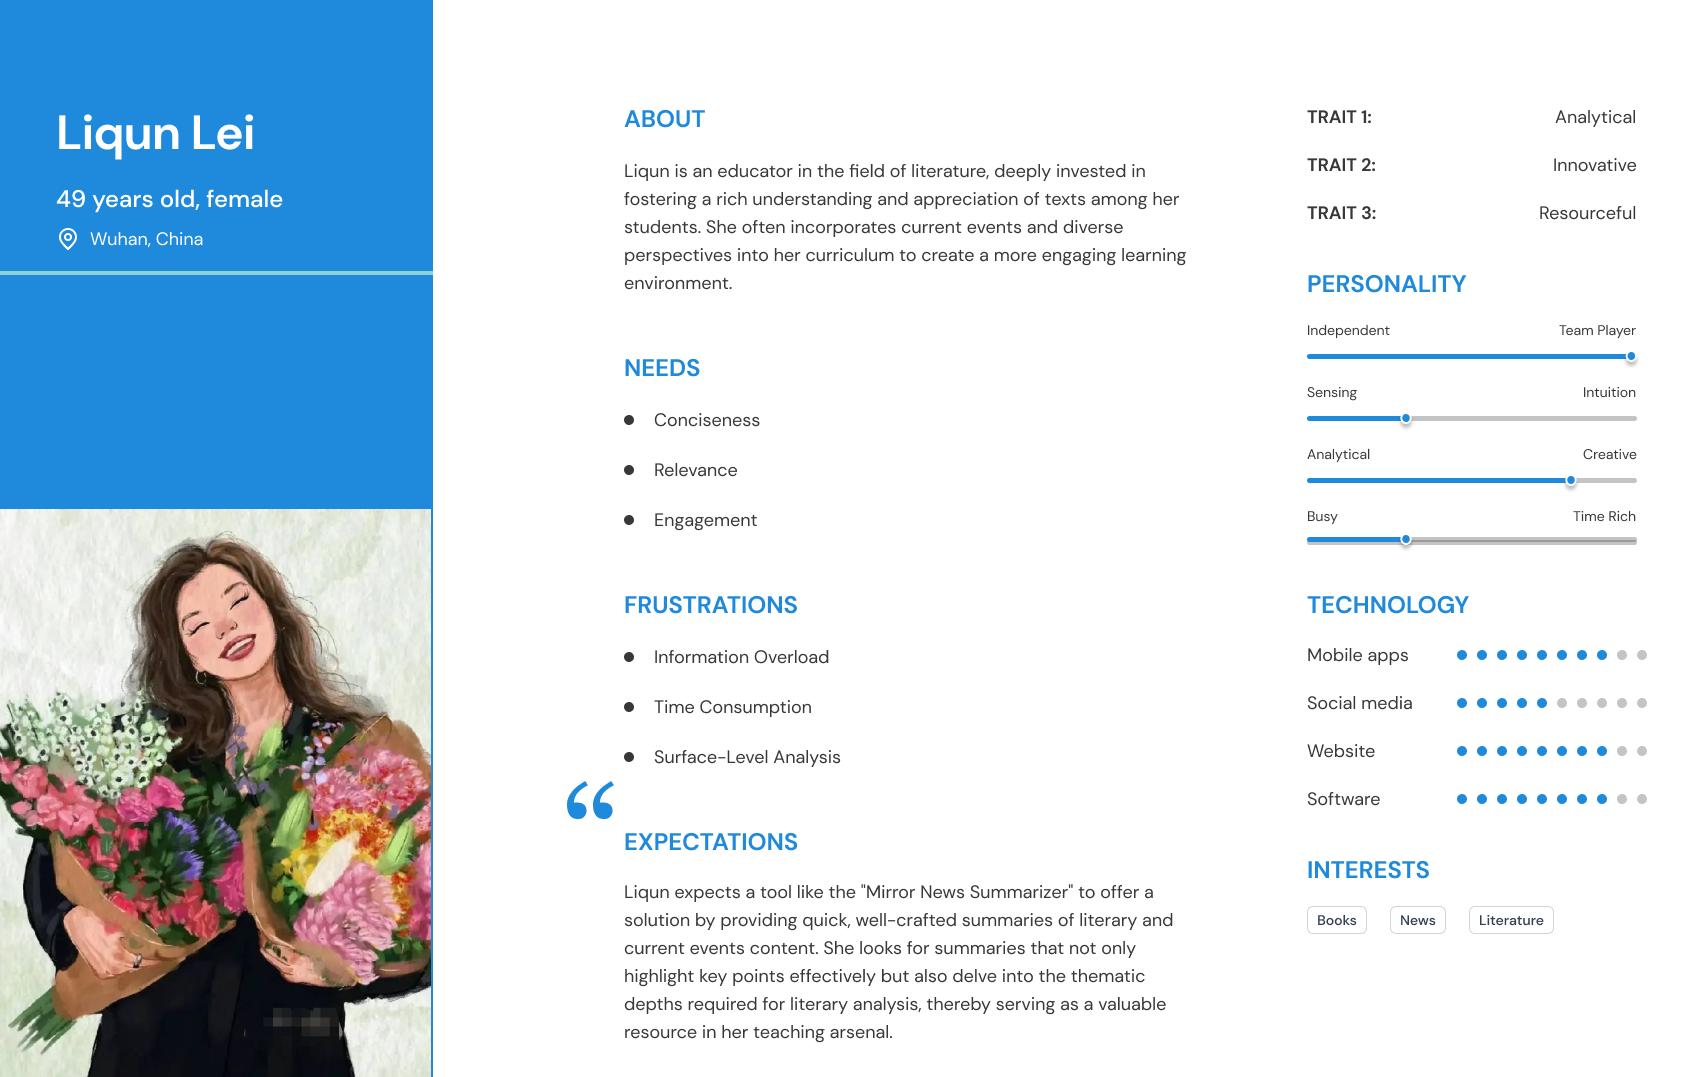
\includegraphics[width=\textwidth]{../persona liqun.png}
    \caption{Persona: Liqun}
    \label{fig:persona-liqun}
\end{figure}

\begin{figure}[H]
    \centering
    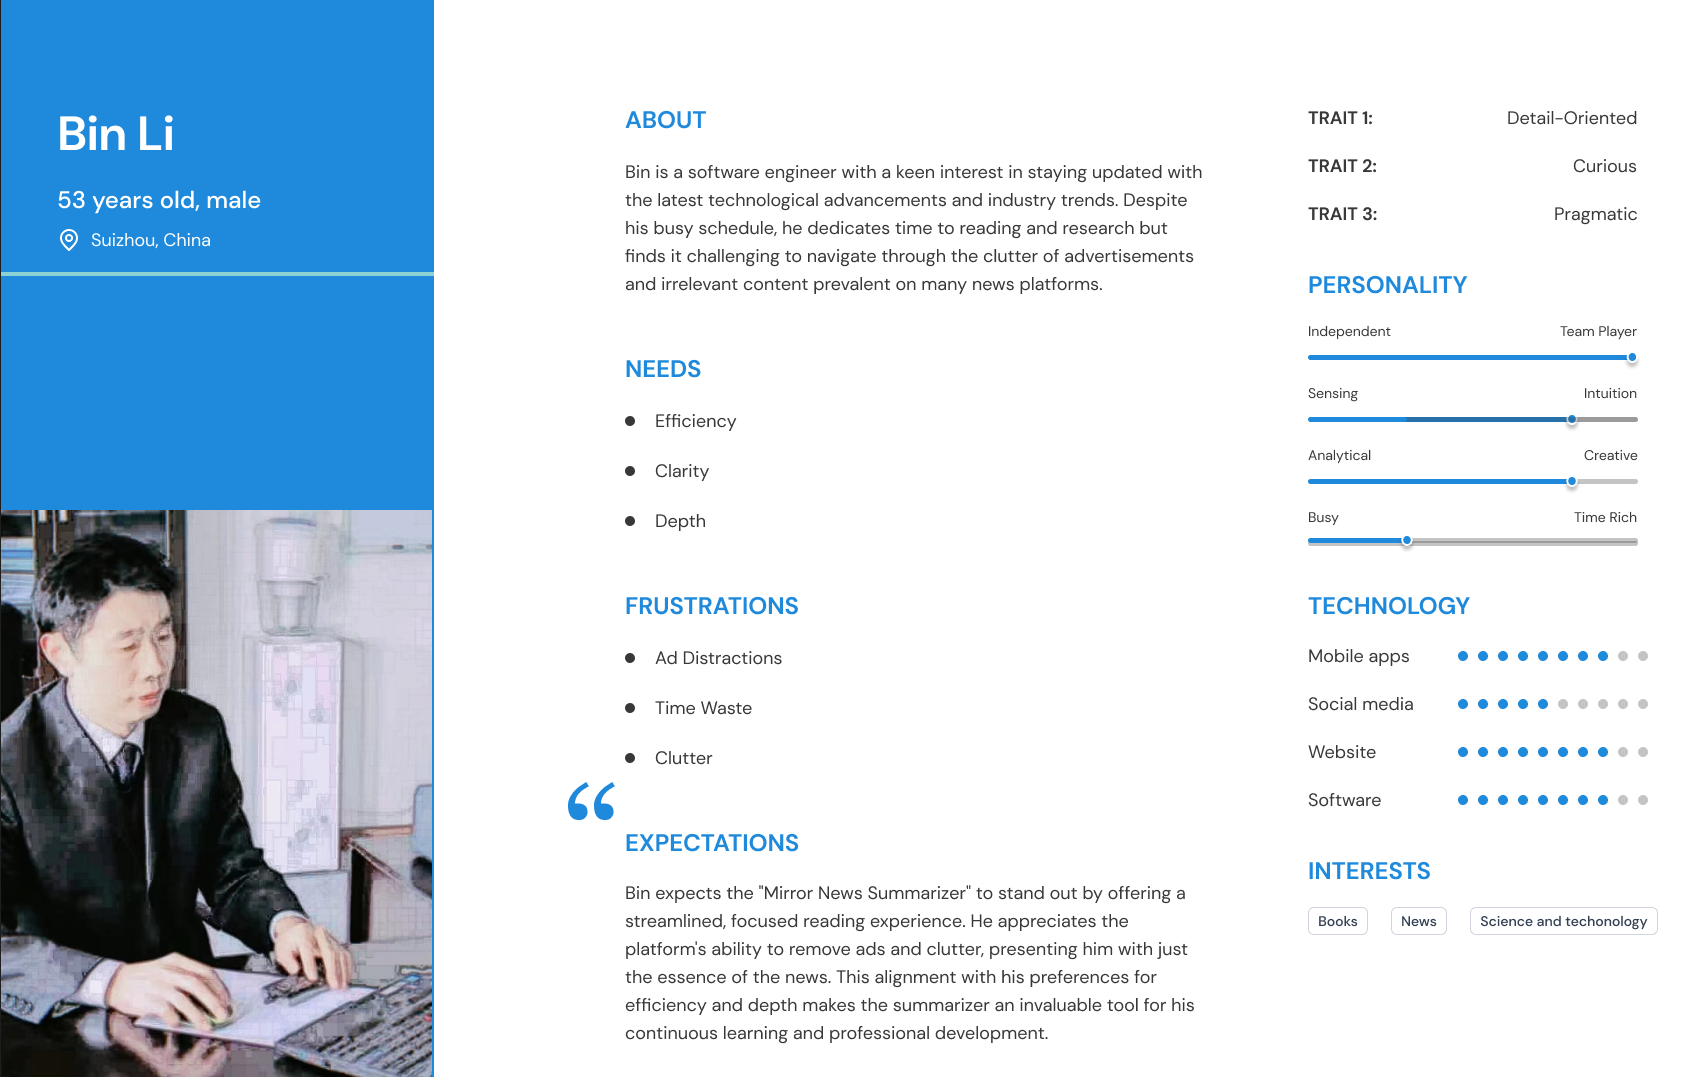
\includegraphics[width=\textwidth]{../persona bin.png}
    \caption{Persona: Bin}
    \label{fig:persona-bin}
\end{figure}

\begin{figure}[H]
    \centering
    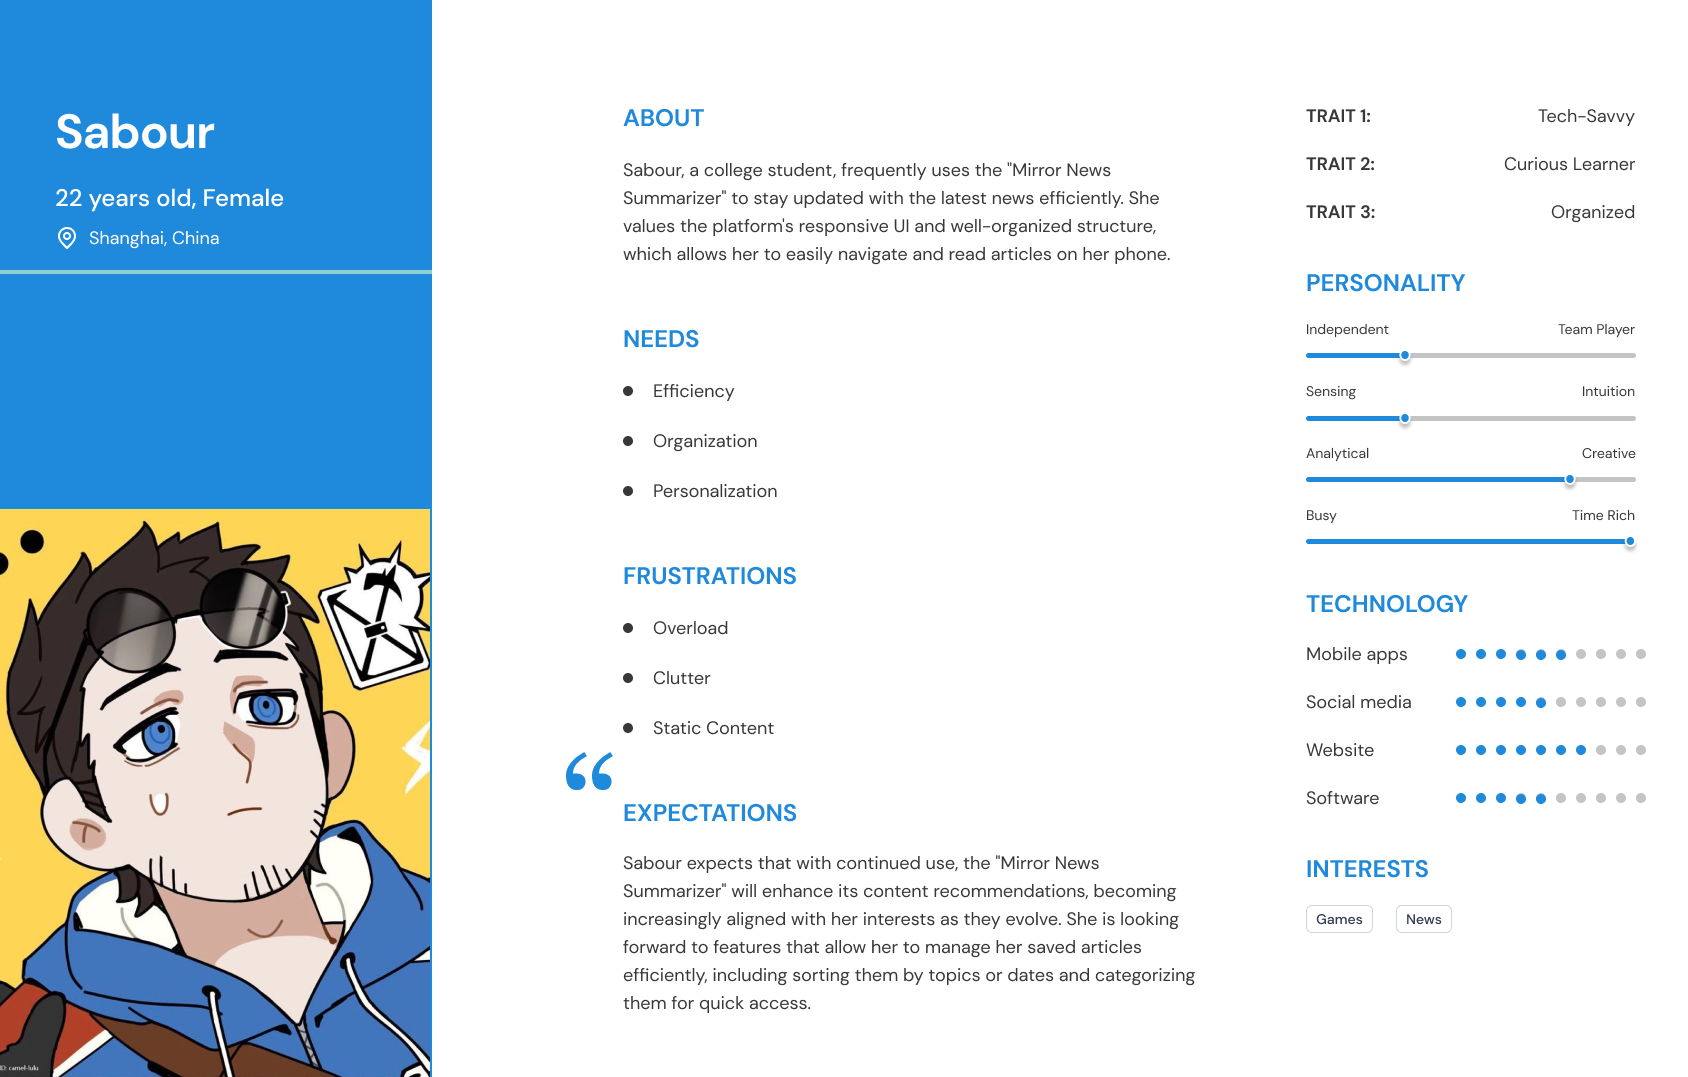
\includegraphics[width=\textwidth]{../persona sabour.png}
    \caption{Persona: Sabour}
    \label{fig:persona-sabour}
\end{figure}

\newpage

\begin{appendices}
    \section{Installation Guide}
    \label{sec:installation_guide}
    
    This appendix provides a concise guide for installing and deploying the "Mirror News Summarizer" on an Amazon Linux server, highlighting both original components and adapted code.
    
    \subsection{Software Requirements}
    \begin{itemize}
        \item Git
        \item Python 3.x
        \item Node.js and npm
        \item Flask
    \end{itemize}
    
    \subsection{Installation Steps}
    
    \paragraph{Step 1: Environment Setup}
    Ensure Git is installed and update your package lists. Clone the project repository and navigate into the project directory:
    \begin{lstlisting}[language=bash]
    sudo yum install git -y
    git clone https://git.cs.bham.ac.uk/projects-2023-24/zxl183.git
    cd zxl183
    \end{lstlisting}
    
    \paragraph{Step 2: Install Dependencies}
    Install Python and npm dependencies:
    \begin{lstlisting}[language=bash]
    python3 -m pip install -r requirements.txt
    curl -o- https://raw.githubusercontent.com/nvm-sh/nvm/v0.39.1/install.sh | bash
    nvm install node
    npm install
    npm run-script build
    \end{lstlisting}
    
    \paragraph{Step 3: Database and Application Setup}
    Prepare the database and start the application server:
    \begin{lstlisting}[language=bash]
    flask db init
    flask db migrate
    flask db upgrade
    npm run build
    flask run --host=0.0.0.0 --port=5000
    # Optionally, to keep the server running in the background:
    nohup flask run --host=0.0.0.0 --port=5000 &
    \end{lstlisting}
    
    \subsection{Code Origin and Attribution}
    \label{subsec:code_origin}
    
    \textbf{Original Work:}
    \begin{itemize}
        \item Static CSS files: \texttt{mirror\_news\_summarizer/static/css}
        \item Templates: \texttt{mirror\_news\_summarizer/template/*.html}
        \item Database Models: \texttt{mirror\_news\_summarizer/user/models.py}
        \item Parser Scripts: \texttt{mirror\_news\_summarizer/parsers}
        \item Core Application: \texttt{app.py}, \texttt{cache\_utils.py}, \texttt{content\_utils.py}
    \end{itemize}
    
    \textbf{Adapted Code:}
    The foundation of this project is based on the \textit{Cookiecutter Flask} template, which provides a structured Flask application layout. Modifications were made to integrate the project's unique features and functionalities.
    
    For detailed installation instructions and code attributions, please refer to the GitHub repository: \\ \href{https://git.cs.bham.ac.uk/projects-2023-24/zxl183.git}{https://git.cs.bham.ac.uk/projects-2023-24/zxl183.git}.
    
\end{appendices}

\end{document}
